\documentclass[11pt,a4paper]{report} 

% Für doppelseitigen Ausdruck (nur bei > 60 Seiten sinnvoll)
% \usepackage{ifthen}
% \setboolean{@twoside}{true}
% \setboolean{@openright}{true} 

% Deutsch
\usepackage[english]{babel}
%\usepackage[ngermusan]{babel} % deutsch und deutsche Rechtschreibung
\usepackage[utf8]{inputenc} % Unicode Text 
\usepackage[T1]{fontenc} % Umlaute und deutsches Trennen
\usepackage{textcomp} % Euro
\usepackage[hyphens]{url}
% statt immer Ab\-schluss\-ar\-beit zu schreiben
% einfach hier sammeln mit -. 
\hyphenation{Ab-schluss-ar-beit}
% Vorsicht bei Umlauten und Bindestrichen
\hyphenation{Ver-st\"ar-ker-aus-gang}
 % eigene Hyphenations, die für das Dokument gelten
\usepackage{amssymb} % Symbole
\usepackage{emptypage} % Wirklich leer bei leeren Seiten
\usepackage[export]{adjustbox} % frickeln mit Bildern
\usepackage{hyperref}
\usepackage{amsmath}              % Mathematische Formeln
\usepackage{amsfonts}             % Mathematische Zeichensätze
\usepackage{amssymb}              % Mathematische Symbole
\usepackage{booktabs}
\usepackage{caption}
\usepackage{tabularx}
\usepackage{subfig}
\usepackage{subcaption}
\usepackage{multirow}
\usepackage{hyphenat}
\usepackage{placeins} % Für \FloatBarrier
\usepackage{changepage}
\usepackage{hyperref}
\usepackage{subcaption}
\usepackage{caption}
\usepackage{graphicx}


%% Fonts, je ein kompletter Satz an Optionen

\usepackage{xcolor} 
% Farben ZUERST DEFINIEREN (NACH xcolor!)
\definecolor{linkblue}{RGB}{0, 0, 100}
\definecolor{linkblack}{RGB}{0, 0, 0}
\definecolor{comment}{RGB}{63, 127, 95}
\definecolor{darkgreen}{RGB}{14, 144, 102}
\definecolor{darkblue}{RGB}{0,0,168}
\definecolor{darkred}{RGB}{128,0,0}
\definecolor{javadoccomment}{RGB}{0,0,240}

\usepackage{hyperref}
\hypersetup{
    colorlinks=true,
    linktoc=all,
    linkcolor=linkblack,
    citecolor=linkblack,
    filecolor=linkblack,
    urlcolor=linkblack
}


% Times New Roman, gewohnter Font, ok tt und serifenlos
%\usepackage{mathptmx} 
%\usepackage[scaled=.95]{helvet}
%\usepackage{courier}

% Palatino mit guten Fonts für tt und serifenlos
\usepackage{mathpazo} % Palatino, mal was anderes
\usepackage[scaled=.95]{helvet}
\usepackage{courier}

% New Century Schoolbook sieht auch nett aus (macht auch tt und serifenlos)
%\usepackage{newcent}

% Oder default serifenlos mit Helvetica 
% ich kann es nicht mehr sehen ...
%\renewcommand{\familydefault}{\sfdefault}

% ein bisschen eine bessere Verteilung der Buchstaben...
\usepackage{microtype}

% Bilder und Listings
\usepackage{graphicx} % wir wollen Bilder einfügen
\usepackage{subfig} % Teilbilder
\usepackage{wrapfig} % vielleicht doch besser vermeiden
\usepackage{listings} % schöne Quellcode-Listings
% ein paar Einstellungen für akzeptable Listings
\lstset{basicstyle=\ttfamily, columns=[l]flexible, mathescape=true, showstringspaces=false, numbers=left, numberstyle=\tiny}
\lstset{language=python} % und nur schöne Programmiersprachen ;-)
% und eine eigene Umgebung für Listings
\usepackage{float}
\newfloat{listing}{htbp}{scl}[chapter]
\floatname{listing}{Listing}

% Seitenlayout
\usepackage[paper=a4paper,width=14.2cm,left=36mm,height=22cm]{geometry}
\usepackage{setspace}
\linespread{1.15}
\setlength{\parskip}{0.5em}
\setlength{\parindent}{0em} % im Deutschen Einrückung nicht üblich, leider

% Seitenmarkierungen 
\newcommand{\phv}{\fontfamily{phv}\fontseries{m}\fontsize{9}{11}\selectfont}
\usepackage{fancyhdr} % Schickere Header und Footer
\pagestyle{fancy}
\renewcommand{\chaptermark}[1]{\markboth{#1}{}}
%\fancyhead[L]{\phv \leftmark}
\fancyhead[RE,LO]{\phv \nouppercase{\leftmark}}
\fancyhead[LE,RO]{\phv \thepage}
% Unten besser auf alles Verzichten
%\fancyfoot[L]{\textsf{\small \kurztitel}}
\fancyfoot[C]{\ } % keine Seitenzahl unten
%\fancyfoot[R]{\textsf{\small Technische Informatik}}


% --- Linienbreiten ---
\renewcommand{\headrulewidth}{0.4pt}  % Linie unter Kopfzeile
\renewcommand{\footrulewidth}{0pt}    % keine Linie über Fußzeile

% Theorem-Umgebungen
\newtheorem{definition}{Definition}[chapter]
\newtheorem{satz}{Satz}[chapter]
\newtheorem{lemma}[satz]{Lemma} % gleicher Zähler wie Satz
\newtheorem{theorem}{Theorem}[chapter]
\newenvironment{beweis}[1][Beweis]{\begin{trivlist}
\item[\hskip \labelsep {\textit{#1 }}]}{\end{trivlist}}
\newcommand{\qed}{\hfill \ensuremath{\square}}

% Quellen teilen
\usepackage{bibtopic} 

% Spezialpakete
\usepackage{epigraph}
\setlength{\epigraphrule}{0pt} % kein Trennstrich

% damit wir nicht so viel tippen müssen, nur für Demo 
\usepackage{blindtext} 

% Zum Zeigen von Fehlern
\usepackage{soul}
\newcommand*\falsch{\st}


\newcommand{\distloss}{\mathcal{L}_{\mathrm{dist}}}
\newcommand{\proploss}{\mathcal{L}_{\mathrm{prop}}}
\newcommand{\reconloss}{\mathcal{L}_{\mathrm{recon}}}
\newcommand{\rigidloss}{\mathcal{L}_{\mathrm{rigid}}}
\newcommand{\isoloss}{\mathcal{L}_{\mathrm{iso}}}
\newcommand{\rotloss}{\mathcal{L}_{\mathrm{rot}}}
%\newcommand{\reconloss}{\mathcal{L}_{\mathrm{recon}}}
\newcommand{\entropyloss}{\mathcal{L}_{\mathrm{entropy}}}
\newcommand{\consistentloss}{\mathcal{L}_{\mathrm{consistent4D}}} % alle Pakete und Einstellungen

% Hier anpassen 
%\newcommand{\welchethesis}{Bachelor}
\newcommand{\welchethesis}{Master}
\newcommand{\thesisofwas}{of Science}
%\newcommand{\studiengang}{Technische Informatik}
% \newcommand{\studiengang}{Medizintechnik}
\newcommand{\studiengang}{Information Technology}
\newcommand{\titel}{Compositional Gaussian Splatting for Multi-Object and Dynamic Scene
Synthesis}
\newcommand{\kurztitel}{Compositional Gaussian Splatting}
\newcommand{\autor}{Luca Hebeda}
\newcommand{\datum}{31. Oktober 2025} % Abgabedatum
\newcommand{\ort}{Mannheim}
\newcommand{\hochschullehrer}{Prof.\ Dr.\ Marcus Vetter}
\newcommand{\zweikorrektor}{M. Sc. Yannick Bukschat}

\begin{document}

% --- FRONTMATTER ---
\pagenumbering{gobble}

\begin{titlepage}
  % Kopf der Seite
  \parbox[b]{80mm}{
    % \textsf würde das Aussehen der ersten Seite ruinieren, 
    % wer will, soll das selbst außen rum machen...
    Department of Information Technology\\
    Course of Studies: \studiengang}
  \hfill
  \parbox[b]{42mm}{
\includegraphics[width=42mm,valign=c,raise=3mm]{images/thmannheimlogo_grey.pdf}}
  \begin{center}
    % rumfiddeln, damit es für 4 Zeilen gerade noch so geht...
    \rule{1\textwidth}{1pt}\\[-3mm]
    \parbox[t][64mm]{110mm}{% 11 cm für Breite 13, ca. 7 für Höhe 6
      \begin{center}
        \vspace{6mm}
        %\Large{Master Thesis}\\[2mm]
        {\begin{spacing}{1.13} \huge \bfseries \titel \end{spacing}}
        \vfill
        \Large{\autor} \\[1mm] % keep space to window
        \ 
      \end{center}
    }
    \rule{\textwidth}{1pt}    
    \vfill    
    {\Large Master Thesis} \\[5mm]
    {\large for the acquisition of the academic degree} \\[5mm]
    {\large \welchethesis\ \thesisofwas} \\[5mm]
    \vfill    
    % \begin{tabular}{ll} % Mitte der Seite
    %   Vorgelegt von & \autor \\
    %   am & \datum \\
    %   Hochschullehrer/in & \hochschullehrer \\
    %   Zweikorrektor/in & \zweikorrektor
    % \end{tabular}    
    \begin{tabular}{ll}
    Submitted by & \autor \\
    on & \datum \\
    Supervisor & \hochschullehrer \\
    Second examiner & \zweikorrektor
    \end{tabular}   
    \vfill
  \end{center}
\end{titlepage}
\cleardoublepage


% Erklärung gemäß der Prüfungsordnung
\thispagestyle{empty}

\subsection*{Written Declaration in Accordance with the Study and Examination Regulations}

  I hereby declare that I have written this thesis independently and have not used any sources or aids other than those indicated.  
  All passages that are taken literally or in substance from other works are identified as such.  

% \subsection*{Schriftliche Versicherung laut Studien- und Prüfungsordnung}

% Hiermit erkläre ich, dass ich die vorliegende Arbeit selbstständig verfasst
% und keine anderen als die angegebenen Quellen und Hilfsmittel benutzt habe.

\vspace{6em}
\noindent\begin{tabular}{p{0.37\textwidth}p{0.56\textwidth}}
\ort, \datum  & \rule{0.56\textwidth}{0.5pt}\\
              & \makebox[1cm]{\ } \autor
\end{tabular}

\vfill

\cleardoublepage


\begin{abstract}
We present a modular and methodologically transparent pipeline for multi-view and temporally consistent synthetic dataset generation based on Gaussian Splatting. 
The framework integrates static 3D Gaussian Splatting (3DGS) and persistent Dynamic 3D Gaussian Splatting (D3DGS) into a unified system that enables reconstruction, export, and recomposition of dynamic multi-object scenes. 
Using a hardware-synchronized 56-camera rig, we capture spatially dense and temporally aligned sequences that serve as the basis for static background reconstruction and dynamic object modeling. 
A dedicated compositing stage allows the exported Gaussian models to be reinserted, duplicated, or combined into novel virtual environments, producing multi-view renderings with synchronized RGB, depth, segmentation, and occlusion annotations. 
Additional modules provide pose estimation, keypoint propagation, and temporal supersampling for motion-consistent supervision signals. 
Qualitative evaluations demonstrate that the pipeline maintains spatial coherence, robust occlusion reasoning, and temporal stability across views and environments. 
The system establishes a practical foundation for controllable 4D dataset generation and for benchmarking methods in dynamic scene understanding.
\end{abstract}


\tableofcontents
\cleardoublepage

\pagenumbering{arabic}
\onehalfspacing

% \linenumbers
\chapter{Introduction}

% Recent advances in neural scene representations have demonstrated that \emph{Gaussian Splatting (GS)} \cite{kerbl3Dgaussians} provides an efficient and photorealistic alternative to Neural Radiance Fields (NeRFs) \cite{mildenhall2021nerf} for multi-view reconstruction. Static 3D Gaussian Splatting (3DGS) methods enable compact and high-fidelity rendering of object-level models, while dynamic extensions such as \emph{Dynamic 3D Gaussians (D3DGS)} \cite{luiten2024dynamic} and several 4D GS variants achieve temporally coherent reconstructions of moving agents. These techniques have established a practical foundation for geometry-aware, image-based rendering and synthetic data generation.

% While these methods are effective for reconstructing individual static or dynamic scenes, less attention has been paid to the problem of \emph{composing} multiple Gaussian-based models into coherent, multi-object, and temporally consistent scenes. Such compositional modeling is highly relevant for dataset generation, simulation, and augmentation, yet it introduces several practical challenges: (i) spatial alignment of exported models across captures, (ii) deterministic occlusion handling in multi-view configurations, and (iii) the generation of temporally consistent multi-modal annotations. Existing approaches such as \emph{Cut-and-Splat} \cite{CutAndSplat2024} explore object-level manipulation but rely on heuristic background placement and do not offer a principled framework for integrating static and dynamic Gaussian models.

% In this paper, we present a modular\emph{composition pipeline} that integrates existing 3DGS and D3DGS models into calibrated multi-view scenes. The system enables the controlled assembly and rendering of multi-object and dynamic scenes while automatically generating synchronized RGB, depth, and instance-level annotations. It includes both \emph{visible} and \emph{complete} instance masks, per-instance bounding boxes, occlusion scores, and candidate 6D placement transforms. In addition, 2D keypoints obtained from a Detectron2 detector \cite{Detectron22020} are temporally propagated to provide motion-consistent supervisory signals for downstream tasks. 
% %Dynamic object reconstructions are supported by \emph{SAM2}-based mask generation \cite{ravi2024sam2}, which ensures temporally stable supervision across all views.

% Because the generated data is fully synthetic, no external ground-truth annotations are available for quantitative comparison. Consequently, our evaluation focuses on qualitative analysis of spatial and temporal consistency across views and over time. We emphasize visual coherence as the primary indicators of system reliability.

% The proposed framework is demonstrated in a controlled, hardware-synchronized 56-camera rig, showing that it produces temporally stable renderings and geometrically consistent multi-modal annotations. By emphasizing compositional reproducibility rather than algorithmic modification, this work bridges the gap between reconstruction-focused Gaussian Splatting methods and practical, multi-object dataset generation workflows.

% \noindent\textbf{Contributions.} The main contributions of this work are summarized as follows:

% \noindent\begin{enumerate}
%     \item A composition pipeline that integrates existing static (3DGS) and dynamic (D3DGS) Gaussian Splatting models into calibrated multi-view scenes, producing synchronized RGB, depth, and instance-level annotations.
%     \item An integrated annotation suite that provides visible and complete instance masks, occlusion scoring, per-instance bounding boxes, candidate 6D placement transforms, and temporally propagated 2D keypoints.
%     \item A qualitative assessment of composition quality and temporal consistency in controlled capture settings, highlighting internal coherence and reproducibility.
% \end{enumerate}


Artificial intelligence has made remarkable progress in understanding and generating visual content \cite{lecun2015deep, krizhevsky2012imagenet}. Modern computer vision systems can recognize objects, estimate depth, and reconstruct three-dimensional scenes from ordinary images \cite{he2017mask, zollhoefer2018state}. Behind these capabilities lies an essential component: the data used to train and evaluate such models \cite{sun2017revisiting}. Most deep learning approaches rely on large collections of labeled data, yet creating high-quality datasets with accurate geometry and temporal consistency remains one of the most expensive and time-consuming parts of research and development \cite{everingham2010pascal, lin2014microsoft}.

In recent years, the representation of visual scenes has shifted from traditional image-based techniques toward neural and hybrid three-dimensional representations. Neural scene representation aims to describe a scene not as a set of disconnected pixels but as a continuous spatial structure that can be viewed from any angle \cite{mildenhall2021nerf}. Methods such as Neural Radiance Fields (NeRFs) have shown that it is possible to reconstruct continuous three-dimensional models from ordinary photographs, although they often require long optimization times and complex rendering processes \cite{barron2021mip}.

Gaussian Splatting has recently emerged as a faster and more transparent alternative \cite{kerbl3Dgaussians}. Instead of relying on deep implicit functions, it models a scene as a collection of Gaussian primitives that represent color, position, and opacity in space. This structure allows real-time rendering while maintaining a high level of detail and realism \cite{fridovich2023k}. Because Gaussian primitives can be easily manipulated and recombined, this approach opens new possibilities for modular scene generation and synthetic data creation \cite{CutAndSplat2024}.

The ability to generate synthetic data is becoming increasingly important for artificial intelligence \cite{tobin2017domain, denninger2019blenderproc}. Real-world datasets are often limited by annotation errors, missing labels, and a lack of variety \cite{dwibedi2017cutpaste}. Synthetic datasets can overcome these problems by providing unlimited, precisely labeled, and perfectly synchronized examples \cite{zanjani2025gaussian}. They are especially valuable in areas where ground-truth information such as depth, motion, or segmentation is difficult to obtain through manual annotation \cite{godard2017unsupervised, bertasius2019maskprop}.
For training robust AI models, it is not only the amount of data that matters but also the quality, consistency, and diversity of the examples. A system that can automatically generate realistic and correctly annotated images from structured three-dimensional representations therefore offers a significant advantage for both academic research and industrial applications.

Despite this potential, most existing methods focus on reconstructing individual static or dynamic scenes \cite{luiten2024dynamic,yang2024deformable}. They do not provide tools for composing multiple objects or actors into coherent multi-view environments with synchronized annotations. In many practical scenarios such as robotics, autonomous systems, or simulation, it is essential to create dynamic scenes that include several interacting elements while maintaining accurate geometry and temporal alignment \cite{CutAndSplat2024}. 

This thesis addresses these challenges by developing a modular pipeline based on static and dynamic Gaussian Splatting. The proposed system allows the reconstruction, composition, and rendering of complex multi-object scenes in calibrated camera setups. It produces synchronized outputs that include color images, depth maps, and instance-level segmentation. The framework also supports additional annotations such as keypoints, occlusion scores, and estimated poses, which makes it a complete solution for generating structured and reproducible synthetic datasets.

The approach emphasizes compositional reliability rather than algorithmic novelty. By integrating existing Gaussian Splatting methods into a unified workflow, it demonstrates how realistic and temporally consistent synthetic data can be created with minimal manual effort. The system thus connects the recent progress in neural scene representation with the practical need for scalable dataset generation.

The remainder of this thesis presents the theoretical background, the design of the proposed pipeline, and a qualitative evaluation of its results. The findings show that Gaussian-based representations can serve not only as tools for rendering but also as a foundation for controllable four-dimensional data generation and future research in dynamic scene understanding. % Externe Datei einbinden
\chapter{Fundamentals}
\label{chap:Fundamentals}

The following chapter explains the fundamental theoretical concepts required to understand this thesis.


\section{Neural Radiance Fields}
\label{sec:Fundamentals_NeRF}

Neural Radiance Fields (NeRF), introduced by Mildenhall et al. \cite{mildenhall2021nerf}, represent a decisive step in the development of novel 3D scene representations.
The approach models a scene implicitly through a neural network that predicts volumetric density and color for a given position and viewing direction.
By employing differentiable rendering techniques and optimizing on multi-view image data, it becomes possible to reconstruct novel viewpoints with high quality.
The underlying idea is illustrated in Figure \ref{fig:nerf_teaser}.

\begin{figure}[h]
    \centering
    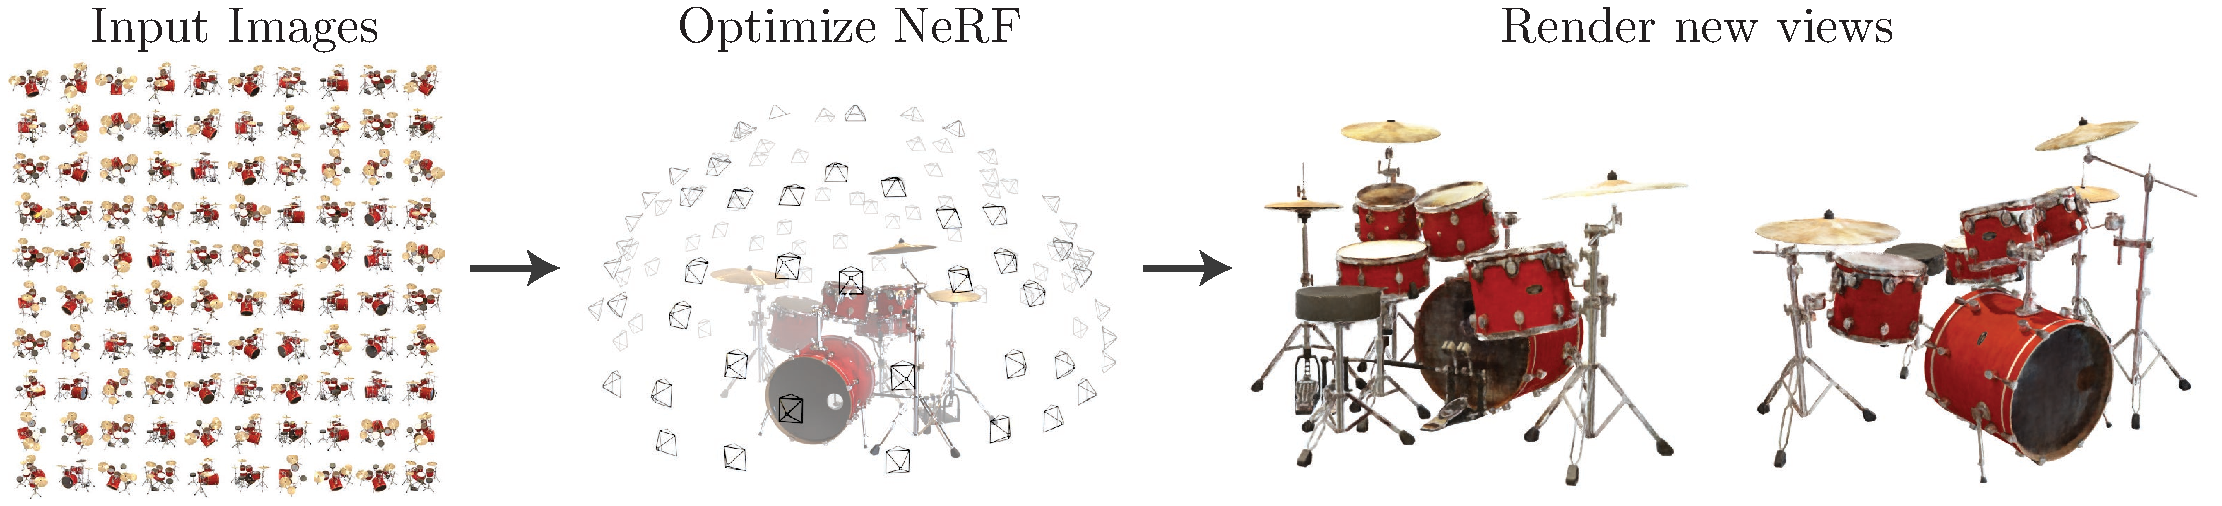
\includegraphics[width=1\linewidth]{Grafiken/Fundamentals/teaser_small.pdf}
    \caption{Core principle of NeRF: A model is optimized from input images and can subsequently generate novel views of the scene (after \cite{mildenhall2021nerf}).}
    \label{fig:nerf_teaser}
\end{figure}

The model receives a 5D vector \((x, y, z, \theta, \phi)\) as input, consisting of the 3D position and the ray direction. 
For each combination of position and direction, the MLP outputs a value for density \(\sigma\) and the associated color \((r, g, b)\).
Rendering is performed by integrating the color and density values estimated by NeRF along the rays projected from the camera into the scene.
The scene representation is optimized by minimizing the photometric error between the rendered and the actual image.
The pipeline is illustrated in Figure \ref{fig:nerf_pipeline}.

\begin{figure}[h]
    \centering
    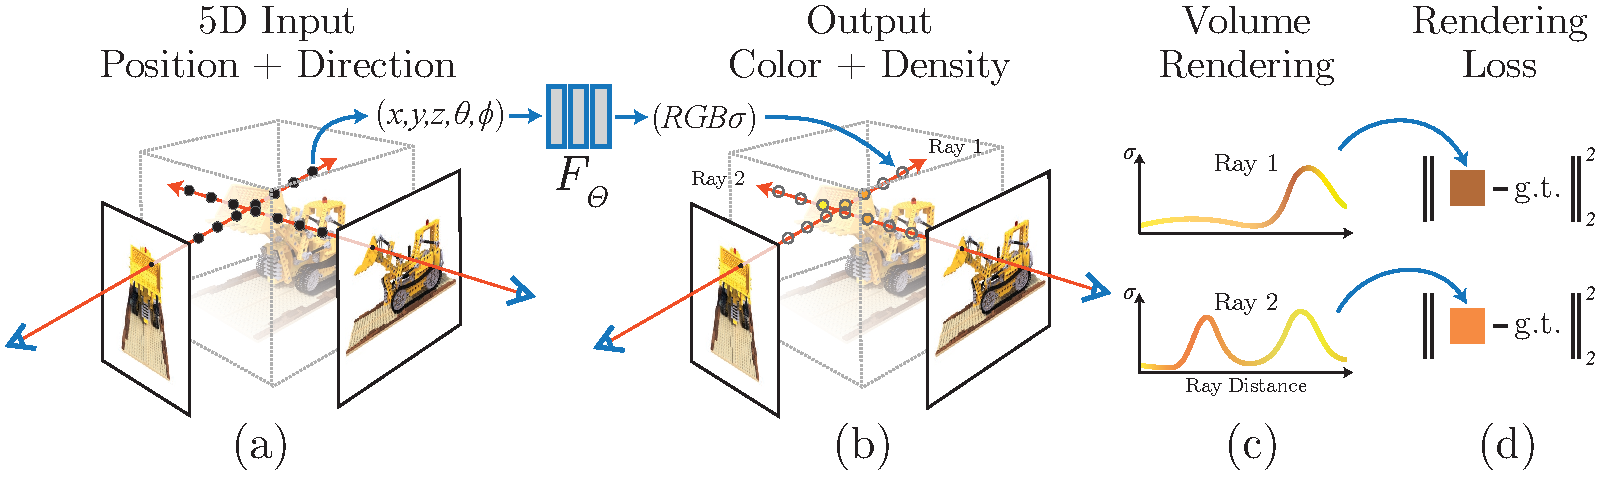
\includegraphics[width=1\linewidth]{Grafiken/Fundamentals/pipeline.pdf}
    \caption{NeRF pipeline: The MLP maps 5D inputs to color and density, which are composed into an image via volumetric rendering (after \cite{mildenhall2021nerf}).}
    \label{fig:nerf_pipeline}
\end{figure}

NeRF enables detailed reconstruction and accurate depiction of complex lighting effects such as reflections and transparencies, making it particularly suitable for photorealistic applications.
Furthermore, the implicit representation ensures consistent multi-view renderings that allow robust synthesis of novel perspectives.


\section{Gaussian Splatting}

While NeRF enables high rendering quality, it suffers from long training times and slow rendering, which is particularly problematic for dynamic scenes and interactive applications.
This motivated the development of alternative representations that are more explicit and efficient.
One of the most significant works in this area is 3D Gaussian Splatting (3DGS) by Kerbl et al. \cite{kerbl3Dgaussians}.
The approach replaces NeRF’s implicit network representation with a set of explicit 3D Gaussians that can be rendered in real time while maintaining high image quality.
An overview of this approach is shown in Figure \ref{fig:overview}, which illustrates the optimization and rendering pipeline of Gaussian Splatting.
The following sections discuss the detailed components of this model to provide a comprehensive understanding of its operation.

\begin{figure*}
\centering
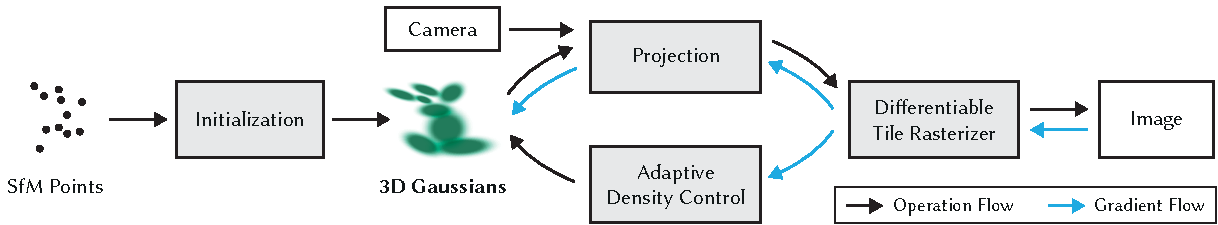
\includegraphics[width=\linewidth]{Grafiken/Fundamentals/overview_01.pdf}
\caption{Optimization and rendering pipeline of Gaussian Splatting: The process begins with a sparse structure-from-motion (SfM) point cloud, which serves as the basis for creating an initial set of 3D Gaussian functions. These Gaussians are refined through iterative optimization, with their density adaptively controlled to ensure accurate scene representation. A fast tile-based rasterizer enables competitive rendering times compared to modern radiance field methods (figure from \cite{kerbl3Dgaussians}).}
\label{fig:overview}
\end{figure*}


\subsection{Scene Representation with 3D Gaussians}

In contrast to NeRF, which requires images from multiple viewpoints as well as camera poses from multi-view stereo (MVS) \cite{schoenberger2016mvs}, Gaussian Splatting is based on a sparse point cloud and camera poses obtained via structure-from-motion (SfM) techniques such as COLMAP \cite{schoenberger2016sfm}.
These points form the basis for creating a set of 3D Gaussian functions, each defined by its position (\(\mu\)), an anisotropic covariance matrix (\(\Sigma\)), an opacity (\(\alpha\)), and spherical harmonic coefficients for color representation.
The 3D Gaussian functions, referred to as \textit{3D Gaussians} throughout this work, are differentiable and can be efficiently projected into 2D splats, allowing fast \(\alpha\)-blending for rendering.
The 3D Gaussians are described by a covariance matrix \(\Sigma\) in world coordinates \cite{kerbl3Dgaussians}, which defines their shape and orientation in 3D space:

\begin{align}
G(x) = e^{-\frac{1}{2} x^T \Sigma^{-1} x}
\end{align}

The matrix \(\Sigma\) describes the extent and correlation of the Gaussian along different axes, providing a compact and flexible representation of the scene.
During rendering, each Gaussian is weighted by its opacity \(\alpha\) to contribute to the final image.


\subsection{Rendering with 3D Gaussian Splatting}

Rendering 3D Gaussians onto the 2D image plane requires several transformations and optimizations to ensure both accuracy and efficiency.
The approach proposed by Zwicker et al. \cite{zwicker2001ewa} provides a robust framework that is central to the 3D Gaussian Splatting technique.

\subsubsection{Projection of 3D Gaussians}

The projection of 3D Gaussians onto the 2D image plane is based on affine transformations and the computation of the covariance matrix in camera coordinates.
The original covariance matrix \(\Sigma\) describes the spatial distribution of the Gaussians in 3D space.
To project it onto the image plane, a view transformation \(W\) is applied, converting the covariance matrix into camera coordinates. The resulting transformed covariance matrix \(\Sigma'\) is computed as follows:

\begin{align}
\Sigma' = J W \Sigma W^T J^T
\end{align}

Where:
\begin{itemize}
    \item \(\Sigma'\): transformed covariance matrix in camera coordinates,
    \item \(W\): view transformation from world to camera coordinates,
    \item \(\Sigma\): original covariance matrix of the 3D Gaussian functions,
    \item \(J\): Jacobian matrix of the affine projection.
\end{itemize}

The Jacobian \(J\) describes the effect of the affine projection on small variations in 3D coordinates.
This transformation maps the spatial distribution of the Gaussians onto the 2D image plane, accounting for the uncertainty of the data points during rendering.

\subsubsection{Simplified Covariance Computation}

Since the transformation described above can be computationally expensive, a simplified approach is often used, based on scaling and rotation matrices.
The covariance matrix \(\Sigma\) can be expressed using a scaling matrix \(S\) and a rotation matrix \(R\):

\begin{align}
\Sigma = R S S^T R^T
\label{eq:calc_sigma}
\end{align}

For optimization, scaling and rotation are stored separately: a 3D vector \(s\) for scaling and a quaternion \(q\) for rotation.
These can easily be converted into matrices and combined, with the quaternion \(q\) being normalized to ensure a valid unit rotation.
This approach allows efficient computation and optimization of the 3D Gaussian Splatting parameters.


\subsection{Optimization}

Optimization in 3D Gaussian Splatting is based on iteratively rendering the scene and comparing it with training images to minimize projection errors of 3D structures on the 2D image plane.
The parameters of the 3D Gaussians, position ($\mu$), covariance matrix ($\Sigma$), opacity ($\alpha$), and color coefficients, are adjusted using stochastic gradient descent.
Opacity \(\alpha\) is constrained to the range [0, 1] using a sigmoid function, while covariance scaling is controlled with an exponential activation function.
The covariance matrix is initially estimated as an isotropic Gaussian model based on the distances to the three nearest points.

The optimization employs a combined loss function:

\begin{align}
\mathcal{L} = (1 - \lambda) \mathcal{L}_1 + \lambda \mathcal{L}_{\text{D-SSIM}}
\label{eq:loss_GS}
\end{align}

Here, \(\mathcal{L}_1\) measures absolute pixel differences between rendered and training images, while \(\mathcal{L}_{\text{D-SSIM}}\) evaluates structural similarity to preserve fine details.
The weighting factor \(\lambda\) balances these two components.

\subsubsection{Adaptive Control of 3D Gaussians}

Adaptive density control, illustrated in Figure \ref{fig:adaptivecontrol}, optimizes the number and distribution of 3D Gaussians.
Every 100 iterations, transparent Gaussians with \(\alpha < \epsilon_\alpha\) are removed, and in regions with large position-dependent gradients, small Gaussians are cloned or large ones are split into smaller ones to accurately represent geometry.
Every 3000 iterations, density is regularized by resetting \(\alpha\) values.
Large Gaussians with excessive influence are removed to maintain efficiency.
This approach allows for a compact and precise scene representation without additional spatial compression.

\begin{figure}[h]
\centering
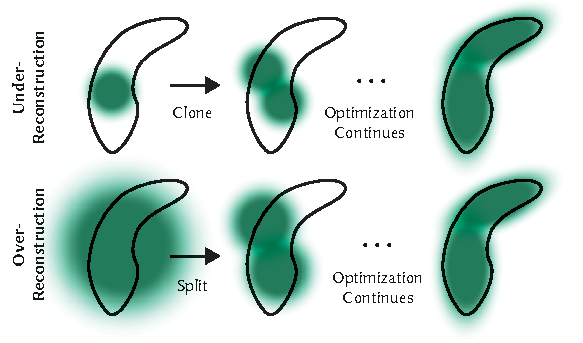
\includegraphics[width=0.5\textwidth]{Grafiken/Fundamentals/density_control_01.pdf}
\caption{Adaptive density control: The top row shows under-reconstruction, where small geometries (black outlines) are supplemented by cloning a Gaussian. The bottom row shows over-reconstruction, where a large Gaussian is split into two smaller ones (after \cite{kerbl3Dgaussians}).}
\label{fig:adaptivecontrol}
\end{figure}


\subsection{Differentiable Rasterizer}

The differentiable rasterizer is central to efficient rendering and optimization of scenes in 3D Gaussian Splatting, as it enables real-time performance and high-quality image synthesis \cite{kerbl3Dgaussians}.

\subsubsection{Tile-based Rasterization Process}

The rasterization projects 3D Gaussians onto the 2D image plane using a view transformation.
The influence of each Gaussian on the pixel grid is computed based on its position (\(\mu\)), covariance (\(\Sigma\)), and opacity (\(\alpha\)).
A tile-based approach divides the image plane into small tiles processed in parallel on the GPU.
The Gaussians are sorted by depth, and their IDs are stored in a list.
Sorting ensures correct color and transparency values during the blending process.

\subsubsection{Rendering and Blending}

During the rendering stage, the individual contributions of all projected Gaussians are accumulated to synthesize the final image. 
Each Gaussian acts as a semi-transparent, view-dependent surface element whose influence on the pixel color is weighted by its opacity and spatial extent in image space. 
This process is realized through \(\alpha\)-blending, a differentiable compositing operation that models light accumulation along the viewing ray.

Formally, the color of a pixel is obtained by sequentially blending all \(N\) Gaussians along the ray in depth order:
\begin{align}
C = \sum_{i=1}^N T_i \alpha_i c_i, \quad \text{with} \quad T_i = \prod_{j=1}^{i-1} (1-\alpha_j)
\end{align}

Here, each term in the summation corresponds to a single Gaussian contribution:
\begin{itemize}
    \item \(C\): final accumulated pixel color,
    \item \(T_i\): transmittance describing how much light passes through all previous Gaussians,
    \item \(\alpha_i\): opacity of the \(i\)-th Gaussian, determining its visibility,
    \item \(c_i\): emitted color of the \(i\)-th Gaussian.
\end{itemize}

The transmittance term \(T_i\) ensures physically correct ordering along the ray, such that closer Gaussians partially occlude those behind them. 
This yields a continuous and differentiable approximation of volumetric compositing, analogous to classical volume rendering but without explicit ray integration.

For each pixel \((u, v)\), the color can be expressed more precisely as:
\begin{align}
I(u, v) = \sum_{i=1}^{N} p_i(u, v; \mu_i^{2d}, \Sigma_i^{2d}) \, \alpha_i \, c_i(d_i) \,
\prod_{j=1}^{i-1} \big(1 - p_j(u, v; \mu_j^{2d}, \Sigma_j^{2d}) \, \alpha_j \big)
\label{eq:projection_3D_gaussians} 
\end{align}

Here, \(p_i(u, v; \mu_i^{2d}, \Sigma_i^{2d})\) denotes the projected 2D Gaussian footprint on the image plane, which determines how strongly each Gaussian contributes to a given pixel.
The term \(c_i(d_i)\) models view-dependent color variations based on the viewing direction \(d_i\), typically parameterized through spherical harmonics. 
Finally, the product term \(\prod_{j=1}^{i-1} (1 - p_j \alpha_j)\) ensures correct visibility by progressively attenuating the contributions of Gaussians located behind others along the ray.


\subsubsection{Backward Pass and Gradient Computation}

Since the entire rendering pipeline is differentiable, gradients of the image reconstruction loss can be propagated back through the rasterization process. 
During the forward pass, the rasterizer stores intermediate quantities such as accumulated transmittance and per-pixel \(\alpha\)-values, which are reused in the backward pass to efficiently compute derivatives. 
This allows for the calculation of gradients with respect to Gaussian parameters including position \(\mu\), covariance \(\Sigma\), opacity \(\alpha\), and color coefficients.

By leveraging these stored buffers, the system avoids redundant recomputation of visibility and blending terms, substantially accelerating optimization. 
This differentiable rasterization design enables end-to-end training through standard gradient descent, directly optimizing the spatial distribution and appearance of Gaussians based on image-space supervision.

\chapter{State of the Art}

\section{Gaussian Splatting for Scene Representation}

Gaussian Splatting has recently emerged as a compact and efficient method for high-quality novel-view synthesis. It provides a practical alternative to volumetric or implicit representations such as Neural Radiance Fields.~\cite{mildenhall2021nerf,barron2021mip,barron2023zipnerf}. 
In GS, a scene is modeled as a set of anisotropic 3D Gaussian primitives, each parameterized by position, covariance, color, and opacity, which are projected and rasterized into image space. 

This representation provides both high rendering fidelity and real-time performance while avoiding the computationally expensive optimization and ray marching inherent to NeRF-based methods~\cite{kerbl3Dgaussians}. 
Because Gaussian primitives can be directly exported, edited, and recombined, 3DGS serves as a convenient intermediate representation for object-level modeling and downstream applications.
Recent studies have extended the approach with semantic and structural grouping of Gaussian primitives.
For instance, Gaussian Grouping~\cite{gaussian_grouping} demonstrated that semantically coherent clusters of Gaussians can be learned jointly with scene geometry, enabling object-level reasoning and segmentation directly in Gaussian space.
Such methods illustrate that Gaussian-based representations can serve as a unified bridge between geometric reconstruction and semantic scene understanding.

\section{Dynamic Extensions of Gaussian Splatting}

Following the success of static 3D Gaussian Splatting (3DGS), a substantial body of work has extended the approach to dynamic scenes. 
Two main paradigms for dynamic extensions have emerged.

The first models temporal evolution explicitly by tracking Gaussian primitives over time. 
Each Gaussian is associated with a trajectory describing its spatial and appearance changes, enabling temporal coherence without retraining. 
Early works such as \textit{Dynamic 3D Gaussians}~\cite{luiten2024dynamic} and \textit{Dynamic Gaussian Marbles}~\cite{stearnsmarbels} follow this paradigm, deriving dense motion fields from the per-Gaussian trajectories. 
More recent variants such as \textit{Deformable 3DGS}~\cite{yang2024deformable} incorporate deformation fields inspired by D-NeRF~\cite{pumarola2021d}, improving temporal smoothness and geometric consistency through explicit regularization. 
These methods preserve modularity and interpretability, allowing reconstructed objects to be reused and exported, but they require careful trajectory regularization to avoid drift.

The second paradigm embeds time directly into the Gaussian representation, treating the primitives as 4D entities with a temporal axis. 
Representative approaches include \textit{4DGS}~\cite{yang2023gs4d}, \textit{SpaceTime Gaussians}~\cite{lispacetimegaussianfeaturesplattingrealtime2024}, and \textit{4D Gaussian Splatting}~\cite{wu20244d}, which employ high-dimensional parameterizations or low-rank factorizations (e.g., K-Planes \cite{fridovich2023k}) to model spatio-temporal changes in position, scale, and orientation. 
These methods achieve globally consistent reconstructions across time but at the cost of increased computational demand and reduced flexibility. 
Once trained, 4DGS models are monolithic and difficult to segment, edit, or recombine, making them less suited for object-centric workflows or dataset generation.


The two dynamic paradigms, trajectory-based and 4D representations, offer complementary trade-offs. Trajectory-based methods, exemplified by D3DGS~\cite{luiten2024dynamic}, prioritize modularity, interpretability, and flexibility, making them well-suited for compositional workflows and synthetic dataset generation. In contrast, 4DGS~\cite{yang2023gs4d} provides globally consistent temporal reconstruction at higher computational cost but with reduced object-level control.  
From the perspective of dataset generation, the trajectory-based approach offers better modularity and reusability. It allows reconstructed objects to be relocated, duplicated, or combined across scenes, which is essential for large-scale synthetic data pipelines. Although four-dimensional representations achieve elegant temporal consistency, their high computational cost and limited flexibility make them less practical for compositional workflows. For this reason, the pipeline developed in this work adopts a trajectory-based dynamic formulation that balances temporal coherence with scalability and per-object control. Methods using 4D Gaussian Splatting are also evaluated as a benchmark for comparison.


\section{Synthetic Compositing and Dataset Pipelines}

Parallel to developments in neural scene representations, a growing body of work addresses synthetic data generation for computer vision. 
Approaches vary from simple image-level composition to physically grounded 3D rendering pipelines. 
Some works create datasets by cutting out segmented objects and pasting them into real backgrounds, optionally guided by depth or matting networks~\cite{Dwibedi2017,Tobin2017,Liu2018,Li2023MattingSurvey}. 
Others synthesize entire virtual scenes using graphics engines such as BlenderProc or Unreal Engine, enabling precise control over scene layout, lighting, and annotations~\cite{Denninger2019,Lee2018}. 
More recent efforts combine learned 3D object models with image-based rendering to generate annotated imagery (RGB, depth, segmentation) for downstream tasks~\cite{Kirillov2023,Bertasius2020,Godard2019,Niu2021}.

However, many compositing pipelines still rely on 2D-level heuristics such as monocular depth estimation or per-frame segmentation, which introduce inconsistencies across viewpoints and over time~\cite{InpaintingLimitations2019,MonoDepthLimitations2018}. 
Promptable segmentation frameworks like SAM~\cite{Kirillov2023} have improved mask quality, but their integration into geometry-aware, multi-view pipelines remains limited~\cite{MaskPropagation2019}. 
Using explicit 3D representations, such as object-level Gaussian models, can mitigate these issues by preserving spatial consistency and enabling deterministic reasoning about what is obscured in different views.

Beyond masks and depth, many dataset pipelines incorporate mid-level cues such as 2D keypoints to provide additional semantic structure. 
Modern detectors based on Mask R-CNN and Detectron2 architectures~\cite{He2017MaskRCNN,Detectron22020} produce accurate joint locations but remain frame-dependent, often suffering from temporal jitter or occlusion failures. 
To improve stability, lightweight propagation and filtering techniques are applied to transfer reliable detections across time~\cite{MaskPropagation2019}. 

\section{Gaussian Splatting for Synthetic Dataset Generation}

Recently, Gaussian Splatting has been explored directly for dataset synthesis. 
\textit{Gaussian Splatting is an Effective Data Generator for 3D Object Detection}~\cite{zanjani2025gaussiansplattingeffectivedata} employs geometric transformations to place 3D Gaussian assets in realistic scenes to improve object detection training. 
Other works have used GS to generate domain-specific datasets, including aerial imagery~\cite{SyntheticDrone2023}, surgical data~\cite{SurgicalGS2023}, and robotic perception scenes~\cite{MobileRobotsGS2024}. 
\textit{Cut-and-Splat}~\cite{CutAndSplat2024} further explores cut-and-paste strategies via Gaussian composition.

These developments highlight the potential of Gaussian Splatting as a foundation for spatially and temporally consistent data generation.
However, existing pipelines often focus on specific applications and lack a general-purpose system that unifies object extraction, segmentation refinement, temporal propagation, and multi-view composition. 
The work presented in this thesis addresses this gap by providing a modular and reproducible framework that integrates static and dynamic Gaussian models into coherent multi-view environments with synchronized multimodal annotations.




\section{Detailed Review of Prominent Dynamic GS Methods}

As previously mentioned, the two main paradigms of dynamic Gaussian splatting offer complementary benefits and trade-offs. The two most prominent methods, Dynamic 3D Gaussian Splatting (D3DGS) ~\cite{luiten2024dynamic} and 4D Gaussian Splatting (4DGS) ~\cite{yang2023gs4d}, are reviewed in detail below to illustrate their underlying principles and differences.



\subsection{Real-time Photorealistic Dynamic Scene Representation and Rendering with 4D Gaussian Splatting}
\label{sec:Real-Time4dgs}

One of the pioneering extensions of 3D Gaussian Splatting to dynamic scenes is the approach by Yang et al.~\cite{yang2023gs4d}. 
This method aims to model the underlying 4D space using 4D Gaussians, treating space and time as a unified construct. 
The complete rendering pipeline is illustrated in Figure~\ref{fig:pipeline_real_time_4D} and explained step by step in the following sections.

\begin{figure*}[ht]
    \centering
    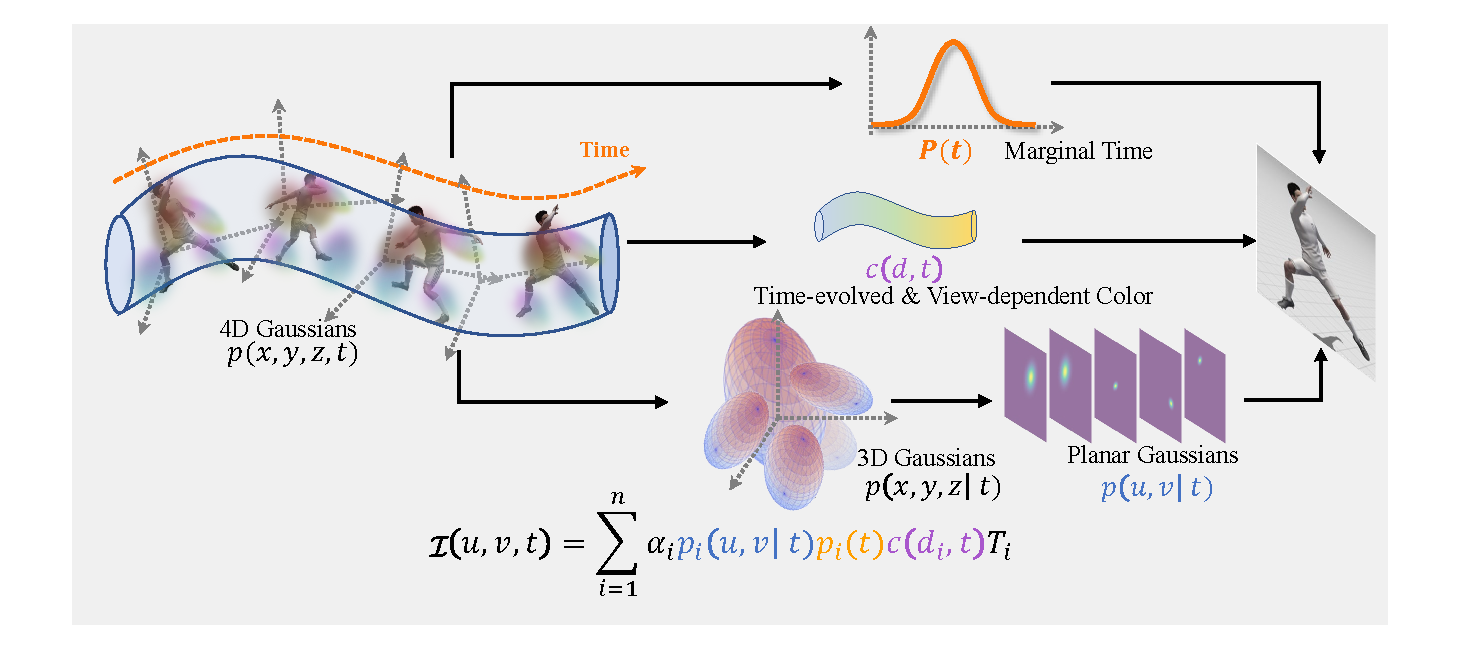
\includegraphics[width=\textwidth]{Grafiken/Fundamentals/pipeline_yang.pdf}
    \caption{The rendering pipeline of the proposed 4DGS method. For a given time \(t\) and view \(I\), each 4D Gaussian is decomposed into a conditional 3D Gaussian and a marginal 1D Gaussian. The conditional 3D Gaussian is then projected onto a 2D splat. Finally, the planar conditional Gaussian, the 1D marginal Gaussian, and the temporally varying, view-dependent color are combined to render the view \(I\) (figure adapted from \cite{yang2023gs4d}).}
    \label{fig:pipeline_real_time_4D}
\end{figure*}

\subsubsection{Extension of the Rendering Equation}

For dynamic scenes, indexing pixels solely by their spatial coordinates \((u,v)\) is insufficient. 
Yang et al.~extend Equation~\ref{eq:projection_3D_gaussians} by an additional timestamp \(t\) to capture the scene dynamics.  
The color \(I(u,v,t)\) of a pixel at time \(t\) is computed by alpha-blending the visible 4D Gaussians:

\begin{align}
I(u,v,t) &= \sum_{i=1}^N p_i(u,v,t) \alpha_i c_i(d) \prod_{j=1}^{i-1} (1 - p_j(u,v,t) \alpha_j)
\end{align}

Here, \(p_i(u,v,t)\) can be further factorized into a conditional probability \(p_i(u,v|t)\) and a marginal probability \(p_i(t)\):

\begin{align}
I(u,v,t) &= \sum_{i=1}^N p_i(t) p_i(u,v|t) \alpha_i c_i(d) \prod_{j=1}^{i-1} (1 - p_j(t) p_j(u,v|t) \alpha_j)
\end{align}

\subsubsection{Scene Representation with 4D Gaussians}

A 4D Gaussian is described by a mean vector \(\mu = (\mu_x, \mu_y, \mu_z, \mu_t)\). 
The definition of the covariance matrix \(\Sigma\) remains identical to the 3DGS formulation~\cite{kerbl3Dgaussians}, factorized via a scaling matrix \(S\) and a rotation matrix \(R\) (cf. Equation~\ref{eq:calc_sigma}).  

The scaling matrix is extended with a temporal scaling factor along the diagonal, resulting in \(S = \mathrm{diag}(s_x, s_y, s_z, s_t)\). 
A rotation in 4D Euclidean space can be constructed from two isotropic rotations, both representable as quaternions. 
This allows anisotropic ellipsoids to rotate freely in space and time.

The left isotropic rotation \(L(q_l)\) and right isotropic rotation \(R(q_r)\) are defined as:

\begin{equation}
R = L(q_l) R(q_r) = 
\begin{pmatrix} 
a & -b & -c & -d \\ 
b & a & -d & c \\
c & d & a & -b \\
d & -c & b & a
\end{pmatrix} 
\begin{pmatrix}
p & -q & -r & -s \\ 
q & p & s & -r \\ 
r & -s & p & q \\ 
s & r & -q & p
\end{pmatrix}.
\label{eq:rotation_matrix}
\end{equation}

\subsubsection{Projection onto the Image Plane}

The conditional 3D Gaussian at a specific time \(p_i(x,y,z|t)\) can now be derived from the properties of the 4D Gaussian:

\begin{align}
\mu_{xyz|t} &= \mu_{1:3} + \Sigma_{1:3,4} \Sigma_{4,4}^{-1} (t - \mu_t) \\
\Sigma_{xyz|t} &= \Sigma_{1:3,1:3} - \Sigma_{1:3,4} \Sigma_{4,4}^{-1} \Sigma_{4,1:3}
\end{align}

After extracting the conditional 3D Gaussians from the 4D representation, the 2D projection can be computed in the same way as for 3DGS.

The marginal distribution \(p_i(t)\) indicates at which times a Gaussian contributes to the scene. 
It can be described by a 1D Gaussian:

\begin{align}
p_i(t) &= \mathcal{N}(t; \mu_4, \Sigma_{4,4})
\end{align}

\subsubsection{Spherical Harmonics for Color Representation}

To model temporal evolution and view-dependent color, spherical harmonics are employed. 
These extend conventional spherical harmonics to account for the temporal dimension. 
The color is represented as a combination of 4D spherical harmonics:

\[
Z_{nlm}(t, \theta, \phi) = \cos\left(\frac{2\pi n}{T} t\right) Y_l^m(\theta, \phi),
\]

where \(Y_l^m\) are the 3D spherical harmonics, \(l\) the degree, \(m\) the order, and \(n\) the Fourier order. 
This enables modeling of temporally varying, view-dependent colors.

% \subsubsection{Evaluation of the Method}

% Compared to previous works, the approach by Yang et al.~\cite{yang2023gs4d} represents a significant advancement, as it enables a consistent representation of dynamic scenes in the space-time continuum while achieving real-time performance. 
% The integration of 4D Gaussians allows for more accurate modeling of temporal dependencies than methods relying solely on 3D representations. 
% However, the original work also highlights limitations: in particular, the increased memory footprint and optimization complexity remain open challenges. 
% Despite these limitations, the method is currently considered a promising approach for photorealistic rendering of dynamic scenes.




\section{Dynamic 3D Gaussians: Tracking by Persistent Dynamic View Synthesis}

One of the foundational works for dynamic Gaussian Splatting is the method proposed by Luiten et al.~\cite{luiten2024dynamic}, which introduces \textit{Dynamic 3D Gaussians} (D3DGS) for representing and tracking dynamic scenes. 
This method forms the basis for the dynamic object reconstruction component of the pipeline developed in this work. 
The following section provides a detailed overview of its representation, physical regularization, and optimization strategy.

\subsubsection{Scene Representation}

In contrast to approaches that model space and time within a shared continuum, D3DGS explicitly tracks Gaussian primitives over time. 
While 3DGS treats Gaussians as static entities in three-dimensional space, D3DGS extends this framework by allowing their positions and orientations to vary across frames. 
Intrinsic properties such as color, opacity, and scale remain fixed, resulting in a representation where Gaussians behave like physical particles undergoing rigid-body motion. 
The method maintains a fixed number of Gaussians per scene rather than dynamically creating or deactivating them over time. 
This consistency facilitates compositional workflows, as objects can be represented and manipulated uniformly across scenes. 
To ensure physically plausible and temporally coherent motion, Luiten et al. augment the model with several regularization terms that encode physical priors.

\begin{figure*}[ht]
    \centering
    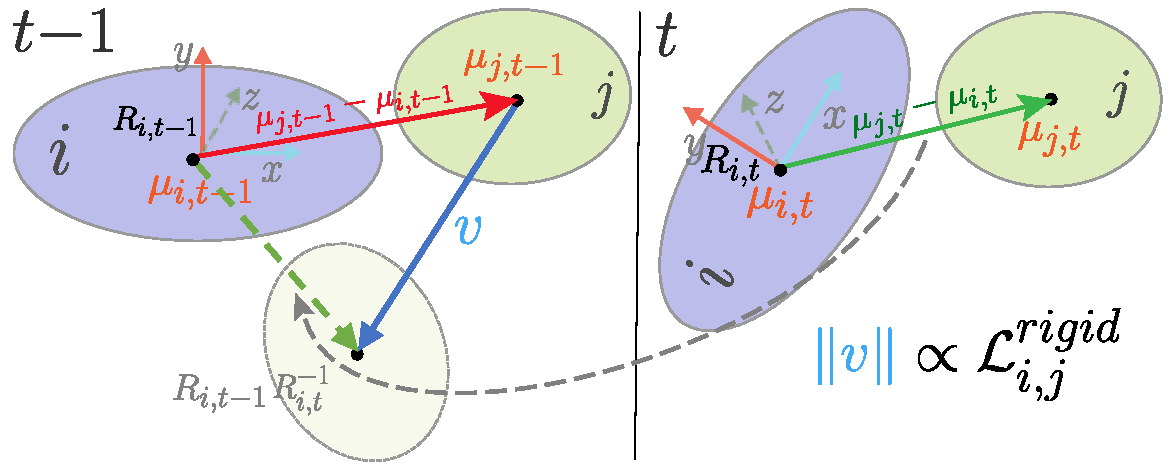
\includegraphics[width=\textwidth]{Grafiken/Fundamentals/loss_fig_luiten.pdf}
    \caption{Schematic illustration of the local rotation similarity loss in D3DGS~\cite{luiten2024dynamic}.}
    \label{fig:loss_fig_luiten}
\end{figure*}

\subsubsection{Physical Regularization}

The physical regularization ensures that local structures move consistently and undergo realistic motion patterns. 
Three principal loss terms are introduced to enforce these constraints.

\paragraph{Local Rigidity Loss}

The rigidity loss enforces that neighboring Gaussians exhibit motion consistent with a local rigid-body transformation. 
For each Gaussian \(i\), its neighbors \(j\) across two consecutive time steps should follow a similar transformation (see Fig.~\ref{fig:loss_fig_luiten}). 
The loss is defined as:
\begin{align}
\rigidloss = \frac{1}{k|S|} \sum_{i \in S} \sum_{j \in \text{k-nn}} w_{i,j} \|(\mu_{j,t-1} - \mu_{i,t-1}) - R_{i,t-1} R_{i,t}^{-1} (\mu_{j,t} - \mu_{i,t})\|^2,
\end{align}
where the weighting factor \(w_{i,j}\) depends on the spatial proximity of two Gaussians in the initial configuration:
\begin{align}
w_{i,j} = \exp \left( -\lambda_w \|\mu_{j,0} - \mu_{i,0}\|^2 \right).
\end{align}
This loss preserves the relative structure of local neighborhoods over time.

\paragraph{Local Rotation Similarity Loss}

In addition to translation, the rotation of neighboring Gaussians should remain consistent. 
To achieve this, a rotation similarity loss measures the difference between the quaternions representing the local motion:
\begin{align}
\rotloss = \frac{1}{k|S|} \sum_{i \in S} \sum_{j \in \text{k-nn}} w_{i,j} \|q_{j,t} q_{j,t-1}^{-1} - q_{i,t} q_{i,t-1}^{-1}\|^2.
\end{align}
This encourages spatially coherent rotational motion across neighboring Gaussians.

\paragraph{Isometry Loss}

The isometry loss stabilizes the distances between Gaussians over time, preventing local neighborhoods from deforming excessively. 
It is defined as:
\begin{align}
\isoloss = \frac{1}{k|S|} \sum_{i \in S} \sum_{j \in \text{k-nn}} w_{i,j} \left| \|\mu_{j,0} - \mu_{i,0}\| - \|\mu_{j,t} - \mu_{i,t}\| \right|.
\end{align}
Compared to the more restrictive rigidity loss, this term acts as a softer constraint, allowing moderate flexibility while maintaining approximately constant inter-Gaussian distances.

\subsubsection{Optimization}

Optimization follows the same principle as static 3DGS and relies on the image reconstruction loss defined in Equation~\ref{eq:loss_GS}. 
Training proceeds sequentially over time steps, leading to a linear increase in computation time with sequence length. 
A major limitation of this formulation is its reliance on dense multi-view supervision: 
if certain viewpoints are missing, Gaussians that become occluded or leave the field of view can no longer be reliably tracked, reducing robustness in scenes with partial visibility.
 % Externe Datei einbinden
%
\chapter{Methodik}

In diesem Kapitel wird die allgemeine Methodik der vorliegenden Arbeit beschrieben.

\section{3D Gaussian Splatting}

Zunächst wird untersucht, ob die neuartige Methode Gaussian Splatting für die 3D-Szenenrekonstruktion im Neural Space Time Lab (NSTL) geeignet ist.
Dazu wird COLMAP als Standardmethode zur Initialisierung mit einer Kalibrierung der Kameraparameter mithilfe von OpenCV verglichen, um Unterschiede in Genauigkeit und Leistung aufzuzeigen.

\subsection{Datensatzvorbereitung}
\label{sec:Datensatzvorbereitung}
Die Datensätze müssen in ein geeignetes Format gebracht werden, um sie im System nutzbar zu machen.

\subsubsection{COLMAP}

Die Bilder werden für COLMAP mithilfe eines bereitgestellten Skripts vorverarbeitet, das Feature Matching durchführt und eine grobe Punktwolke für die Initialisierung der 3D-Gaussians erstellt. 
Anschließend werden die Bilder mit den geschätzten Kameraparametern auf eine optimale Pinhole-Kamera entzerrt.

\subsubsection{OpenCV}
Die Vorverarbeitung mit OpenCV ist aufgrund der manuellen Kalibrierung zeitaufwendiger. 
Die Kameras im NSTL wurden zuvor intrinsisch und extrinsisch kalibriert, und diese Kalibrierung wird nun zur Entzerrung der Bilder verwendet.

\subsubsection{Entzerrung}
Gaussian Splatting setzt voraus, dass der Hauptpunkt der Kameramatrix im Bildzentrum liegt. Die Kameras im NSTL weisen jedoch einen versetzten Hauptpunkt von bis zu 40 Pixeln auf, was zu Projektionsfehlern führen kann. Mithilfe der OpenCV-Funktion newOptimalCameraMatrix mit alpha=0 werden die Bilder entzerrt, sodass der Hauptpunkt zentriert wird, ohne ungültige Bildbereiche hinzuzufügen. Dabei gehen jedoch an den Rändern Teile der Bildinformationen verloren. Diese Korrektur ist entscheidend, um die Konsistenz in Multi-View-Systemen zu gewährleisten und die räumliche Kohärenz in Gaussian Splatting zu erhalten. Die entzerrten Bilder und aktualisierten Kameramatrizen werden für das Training gespeichert.

\subsection{Camera Metadata in Json Format}
Nach der Vorverarbeitung werden die Kamerametadaten in einer transforms.json-Datei gespeichert, die Gaussian Splatting zum Laden der Daten nutzt. Diese JSON-Struktur enthält für jeden Frame den Dateipfad des Bildes, eine 4x4-Transformationsmatrix aus der extrinsischen Kalibrierung (Welt-zu-Kamera-Transformation) sowie die im vorherigen Schritt aktualisierte 3x3-Kameramatrix.

\subsection{Trainingsansätze}


Zur Validierung der Methode des 3D Gaussian Splatting wurde zunächst die Szene \textit{bicycle} aus dem Mip-NeRF 360 Datensatz \cite{barron2021mip} verwendet, um die im Referenzpaper \cite{kerbl3Dgaussians} angegebenen Ergebnisse zu reproduzieren. Diese Szene wurde gewählt, da sie im Paper ausführlich beschrieben ist und eine Vergleichbarkeit der Metriken wie SSIM, PSNR und LPIPS ermöglicht. Das Training wurde mit den Standardparametern der Methode durchgeführt und die Ergebnisse des Trainings nach 30.000 Iterationen miteinander verglichen.
Die Ergebnisse zeigten eine hohe Übereinstimmung mit den Literaturwerten, wie im Ergebnis-Teil (Kapitel~\ref{chap:Ergebnisse}) detailliert beschrieben.

Nach erfolgreicher Validierung wurden Experimente mit einem neu aufgenommenen Datensatz aus dem Neural Space Time Lab (NSTL) durchgeführt. Dieser Datensatz wurde zweifach vorbereitet.
Zum einen mit der COLMAP-Methode und zum anderen mit OpenCV, um die Auswirkungen der unterschiedlichen Kalibrierungsansätze auf die Rekonstruktionsqualität zu vergleichen. 
Die Ergebnisse zeigten, dass die Rekonstruktionen in der Region of Interest (ROI) im Zentrum des Raumes nahezu identisch waren, mit nur geringfügigen Unterschieden in den Metriken (siehe Kapitel~\ref{chap:Ergebnisse}).

Die Kalibrierung mit OpenCV erwies sich jedoch als vorteilhafter für die Anwendung im NSTL. 
Für die Kalibrierung mit OpenCV nutzt das Institut eine deterministische Kalibrierung mithilfe eines Charucoboards zur Bestimmung der intrinsischen und extrinsischen Kameraparameter.


Dadurch wird ein Koordinatensystem in realen Maßeinheiten (in diesem Fall Meter) definiert, das eine präzise und für den Menschen nachvollziehbare Zuordnung räumlicher Positionen ermöglicht.
Diese Eigenschaft ist besonders wichtig für die Integration mit anderen Systemen im Neural Space Time Lab (NSTL), wo exakte räumliche Beziehungen für die Multikameradaten erforderlich sind. 
Im Gegensatz dazu verwendet COLMAP eine Struktur-aus-Bewegung (SfM)-Methode, die Kameraparameter und ein synthetisches Koordinatensystem durch Feature Matching und iterative Optimierung schätzt. 
Dieses Koordinatensystem ist nicht in realen Maßeinheiten definiert und erfordert eine nachträgliche Skalierung, die zusätzliche Unsicherheiten in die Rekonstruktion einführt. 
Die deterministische Kalibrierung mit OpenCV und dem Charucoboard gewährleistet eine höhere Genauigkeit und Konsistenz über verschiedene Szenen hinweg, da sie keine szenenspezifischen Abhängigkeiten der Kameraparameter aufweist. 

Obwohl COLMAP in vielen 3D-Rekonstruktionsanwendungen qualitativ hochwertigere Ergebnisse liefern kann, wird OpenCV im NSTL-Kontext bevorzugt. Dies liegt an der robusten und reproduzierbaren Kalibrierung, die eine direkte Übertragbarkeit der Kameraparameter auf verschiedene Szenen ermöglicht und die Notwendigkeit nachträglicher Anpassungen minimiert.
Daher stellt OpenCV eine stabilere und für die Anforderungen des NSTL besser geeignete Grundlage für die weitere Untersuchung von 3D- und 4D-Gaussian-Splatting-Anwendungen dar.



\section{Darstellung von neuen Ansichten und Tiefenbildern}
\label{sec:new_views_depth}

Ein wesentlicher Vorteil des 3D Gaussian Splatting besteht darin, dass die zugrunde liegende Repräsentation nicht an die diskreten Kamerapositionen der Trainingsdaten gebunden ist. 
Da die Szene als kontinuierliche Punktwolke in Form anisotroper Gaussians modelliert wird, können beliebige neue Kamerapositionen definiert und für die Erzeugung von Ansichten genutzt werden. 
Dies ermöglicht es, auch Perspektiven zu rendern, die im Trainingsprozess nicht enthalten waren. 
Abbildung~\ref{fig:cam_setup} zeigt hierzu exemplarisch die Positionen der Trainingskameras, die die Grundlage für die Optimierung des Modells bilden. 
Darüber hinaus lassen sich neue Kamerapfade definieren, um Ansichten aus frei gewählten Positionen zu generieren. 
Dies eröffnet den Zugang zu einer Vielzahl zusätzlicher Darstellungen, die insbesondere für Visualisierungen und qualitative Analysen von Vorteil sind. 

Neben Farbbildern können durch den Rasterisierungsprozess auch Tiefenkarten erzeugt werden. 
Diese stellen die geometrische Struktur der rekonstruierten Szene dar und liefern damit eine zusätzliche Modalität zur Analyse der Rekonstruktion. 
Tiefenbilder sind vor allem für Anwendungen in der Robotik oder für die Integration mit weiteren Sensorsystemen von Bedeutung, da sie die Lageinformation einzelner Strukturen im Raum unmittelbar erfassbar machen. 
Ein Beispiel für eine generierte Tiefenkarte ist in Abbildung~\ref{fig:depth_example} dargestellt.

Die detaillierte Auswertung der erzeugten Bilder erfolgt im Ergebnisteil dieser Arbeit. 
Zusätzliche Darstellungen von Ansichten außerhalb der Trainingskameras sowie von Tiefenkarten sind im Anhang enthalten, um die Vielseitigkeit der Methode zu illustrieren, ohne den Ergebnisabschnitt durch eine Vielzahl visueller Beispiele zu überfrachten.

% \begin{figure}[h]
%     \centering
%     \includegraphics[width=0.7\linewidth]{bilder/methods/camera_setup.png}
%     \caption{Schematische Darstellung der verwendeten Trainingskameras: Die kontinuierliche Repräsentation der Szene erlaubt es, beliebige zusätzliche Ansichten durch neue Kamerapositionen zu erzeugen.}
%     \label{fig:cam_setup}
% \end{figure}

% \begin{figure}[h]
%     \centering
%     \includegraphics[width=0.7\linewidth]{bilder/methods/depth_example.png}
%     \caption{Beispiel einer aus 3D Gaussian Splatting generierten Tiefenkarte: Neben Farbbildern lassen sich auch geometrische Informationen in Form von Tiefenbildern extrahieren.}
%     \label{fig:depth_example}
% \end{figure}
















\section{4D Gaussian Splatting}

Im vorherigen Abschnitt wurde die Methode des 3D Gaussian Splatting vorgestellt und ihre Anwendbarkeit für die Rekonstruktion statischer Szenen im Neural Space Time Lab (NSTL) validiert.
Das NSTL ermöglicht jedoch auch die Aufnahme zeitsynchroner Daten, wodurch die zeitliche Komponente in die Rekonstruktion einbezogen werden kann.
Für die Modellierung dynamischer Szenen ist daher eine Erweiterung auf 4D Gaussian Splatting erforderlich, das die Bewegung und Veränderungen über die Zeit hinweg berücksichtigt. Die Vorverarbeitung der Daten bleibt dabei identisch zu 3D Gaussian Splatting.
Die Bilder werden entzerrt, und die Kamerametadaten werden im JSON-Format strukturiert. Zusätzlich werden nun Zeitstempel zu den Kameradaten hinzugefügt, um die zeitlichen Abstände zwischen den Bildern eindeutig zu definieren. 
Diese Zeitstempel bilden die Grundlage, um die Multikameradaten des NSTL in eine kohärente, zeitliche Rekonstruktion zu überführen.
Da verschiedene Ansätze zur Modellierung dynamischer Szenen existieren, wurde eine Methode gesucht, die sowohl die räumliche als auch die zeitliche Kohärenz effizient abbildet. 


\section{4DGS by Wang et al.}

Die Methode von Wang et al. \cite{yang20244dgs} wurde aufgrund ihrer überlegenen Renderinggeschwindigkeit und Rekonstruktionsqualität ausgewählt. Im Vergleich zu anderen Ansätzen, wie etwa Wu et al. \cite{wu20244d}, zeigte sie in der Literatur bessere Ergebnisse bei gängigen Metriken wie PSNR und SSIM sowie eine bis zu dreifache Renderinggeschwindigkeit. Diese Eigenschaften machen sie besonders geeignet für die Erzeugung neuer Daten aus dynamischen Szenen im Neural Space Time Lab (NSTL). Im Folgenden werden die Trainingsansätze, Verbesserungsansätze und ein speziell für den NSTL entwickelter Ansatz für das Training mit festem Hintergrund vorgestellt.

\subsection{Validierung der Methode}
Zur Validierung der Methode von Wang et al. wurde ein ähnlicher Ansatz wie bei 3D Gaussian Splatting verfolgt, um die Reproduzierbarkeit der im Referenzpaper \cite{yang20244dgs} angegebenen Ergebnisse zu überprüfen. Dazu wurden zwei Testdatensätze verwendet: eine synthetische Szene aus dem D-NeRF-Datensatz \cite{pumarola2020dnerf}, bestehend aus 100 Frames mit einer dynamischen Figur, und eine Szene aus dem Plenoptic-Datensatz \cite{li2022neural}, die 50 Frames mit komplexen Bewegungen umfasst.
Beide Datensätze wurden mit den Standardparametern der Methode trainiert, welche in den zugehörigen yaml-Files abgelegt werden. 
Die Ergebnisse zeigten eine hohe Übereinstimmung mit den Literaturwerten, wie im Ergebnis-Teil (Kapitel~\ref{chap:Ergebnisse}) detailliert beschrieben.


\subsection{Datensätze aus dem NSTL}

Anschließend wurde die Methode auf einen neu aufgenommenen Datensatz angewendet.
Der erste Datensatz umfasste 200 Frames, welche mit 30 FPS aufgenommen wurden und somit eine Zeitspanne von 6.6 Sekunden abbildet.
Die Szene zeigt eine Person, die die Arme auf und ab bewegt und sich währenddessen im Kreis dreht. 
Zuerst wurden Experimente zur Analyse der Qualität mit verschiedener Anzahl an Gaussians durchgeführt. 
Dabei wurde schnell ersichtlich, dass die Qualität stark von der Anzahl an Gaussians abhängig ist.
In \ref{sec:results_4dgs} sind die Ergebnisse dazu dargestellt.

Leider konnte aufgrund von Hardwarebegrenzungen die Anzahl der Gaussians nicht weiter erhöht werden, da sonst der Speicher überläuft und das Training beendet.
Deshalb wurde die Länge der Szene auf ein Viertel gekürzt und nur noch die ersten 50 Frames und somit 1.6 Sekunden betrachtet.
Dies reduziert die Komplexität der Szene weiter, da deutlich weniger Zeitschritte modelliert werden müssen und somit in wichtigen, sich schnell bewegenden Bereichen wie den Händen der Person mehr Gaussians genutzt werden können als zuvor mit der kompletten Szene.



\subsection{Analyse der temporalen Redundanz}

Das Paper von Yuan et al.~\cite{yuan20251000fps4dgaussian} zeigte, dass die hohen Speicherkosten der Methode von Wang et al.~\cite{wang20234dgs} maßgeblich durch kurzlebige Gaussians verursacht werden, selbst in Szenen mit überwiegend statischem Hintergrund. 
Solche kurzlebigen Gaussians tragen oft nur für wenige Frames zur Bildinformation bei und verschwinden anschließend wieder, wodurch redundante Daten entstehen, die den Speicherverbrauch erhöhen, ohne einen nachhaltigen Beitrag zur Szenenrepräsentation zu leisten.  

\subsubsection{Empirische Analyse}  
Zuerst wurde untersucht, ob die Aussagen aus dem Paper auch in den Modellen aus dem NSTL-Datensatz auftreten.
Zur Untersuchung wurde das finale Modell mit den 50 Frames des NSTL-Datensatzes analysiert.  
In Abb.~\ref{fig:gaussians_percentage} wird der Wert der Kovarianz dargestellt, der dafür verantwortlich ist, wie lange ein Gaussian innerhalb einer Szene aktiv ist und somit zum gegebenen Zeitschritt beiträgt.
Dabei ist klar ersichtlich, dass der Großteil der Gaussians einen sehr geringen Wert für die zeitliche Kovarianz aufweist und somit nur in einzelnen aufeinanderfolgenden Zeitschritten aktiv ist. 
Abb.~\ref{fig:gaussians_active} zeigt, dass das aktive Set an Gaussians nur etwa 20\% der Gesamtheit ausmacht und somit 80\% der Gaussians nicht zum aktuellen Zeitschritt beitragen.

Da die Metriken die gleichen Charakteristika zeigen wie im Paper beschrieben, wurde der Spatial-Temporal Score aus dem Paper nachimplementiert, um ihn nutzbar zu machen und somit das Modell effizienter zu gestalten.
Dadurch stehen mehr Rechenressourcen für noch unterrekonstruierte Bereiche der Szene zur Verfügung.
Da keine offizielle Implementierung vorhanden ist, wurde sich an früheren Arbeiten orientiert.

\subsubsection{Spatial Score}  
Um den visuellen Beitrag eines Gaussians $g_i$ zu einem gegebenen Zeitpunkt zu messen, wurde der Spatial Score entwickelt.
Der Spatial Score aggregiert den Strahlenbeitrag eines Gaussians über alle Strahlen $r$ und über alle Eingabebilder zu einem Zeitpunkt:  
\[
S_i^S = \sum_{k=1}^{NHW} \alpha_i \prod_{j=1}^{i-1} (1 - \alpha_j)
\]
wobei $\alpha_i \prod_{j=1}^{i-1} (1 - \alpha_j)$ den Beitrag des $i$-ten Gaussians zur finalen Farbe gemäß Alpha-Komposition widerspiegelt.
Bei der Implementierung wurde sich stark an \emph{lightgaussian} orientiert.
\emph{Lightgaussian} implementiert den Spatial Score für 3D Gaussian Splatting im tile-based Rasterizer, um eine effiziente Berechnung des Spatial Scores zu ermöglichen.
Die Implementierung im Rasterizer konnte somit fast vollständig übernommen und lediglich für den 4D-Fall erweitert werden.

\subsubsection{Temporal Score}  
Entscheidend für die Bewertung der Kurzlebigkeit der Gaussians ist der Temporal Score.
Er gibt Gaussians, die nur kurze Zeit zur Szenenrepräsentation beitragen, einen entsprechend schlechten Score.
Die zeitliche Stabilität wird durch die zweite Ableitung der temporalen Opazitätsfunktion $p_i(t)$ erfasst:
\[
p_i^{(2)}(t) = \left( \frac{(t - \mu_t)^2}{\Sigma_t^2} - \frac{1}{\Sigma_t} \right) p_i(t)
\]
Zur Normierung in das Intervall $(0, 1)$ wird die $\tanh$-Funktion angewendet, woraus der \emph{Temporal Variation Score} $S_i^{TV}$ resultiert:
\[
S_i^{TV} = \sum_{t=0}^{T}  \frac{1}{\left( 0.5 \cdot   \tanh(\lvert p_i^{(2)}(t) \rvert) + 0.5 \right)}
\]
Zusätzlich wird das Volumen des 4D-Gaussians berücksichtigt und normalisiert:
\[
\gamma(S_{4D}) = \text{Norm}(V(S^{4D}))
\]
Der finale \emph{Temporal Score} ergibt sich zu:
\[
S_i^T = S_i^{TV} \cdot \gamma(S_i^{4D})
\]

\subsubsection{Spatial-Temporal Score}  

Der \emph{Spatial-Temporal Variation Score} $S_i$ kombiniert beide Metriken:
\[
S_i = \sum_{t=0}^{T} S_i^T \cdot S_i^S
\]
Dadurch lassen sich Gaussians identifizieren, die sowohl einen hohen visuellen Beitrag als auch eine hohe zeitliche Persistenz aufweisen.

\subsubsection{Training}
Nach der Implementierung konnte der neue Spatial-Temporal Score während des Trainings verwendet werden. 
Zunächst ging es darum zu validieren, wie das Pruning der Gaussians die Ergebnisse der Rekonstruktion beeinflusst.
Dazu wurde zunächst, wie im Paper beschrieben, das Pruning erst nach der vollständigen Densification durchgeführt, wobei Gaussians mit einem schlechten Spatial-Temporal Score entfernt wurden.
Anschließend wurde ein Training gestartet, bei dem das Pruning bereits während der Densification stattfand.
Dies sollte das Ziel haben, Gaussians mit einem schlechten Score frühzeitig zu entfernen und durch neue mit einem besseren Score zu ersetzen.
Die Bewertung der Effektivität dieser Verfahren und deren Einfluss auf Speicherverbrauch und visuelle Qualität erfolgt in Abschnitt~\ref{pruning_results}.


\subsubsection{Eigener Tennis-Volley-Datensatz}

Um den Einfluss redundanter Hintergrund-Gaussians auf Speicherverbrauch und Bildqualität besser zu kontrollieren, wurde ein zusätzlicher Datensatz aufgenommen. 
Dabei wurde der Aufnahmeort gezielt vereinfacht: Der Raum wurde aufgeräumt, der Vorhang geschlossen und auf weitere Personen verzichtet. 
Dadurch sollte vermieden werden, dass Gaussians auf Bereiche außerhalb der eigentlichen Szene verteilt werden und somit unnötig Speicher beanspruchen.

Das Training erfolgte mit denselben Parametern und Evaluationsmetriken wie in den vorherigen Experimenten, sodass die Ergebnisse konsistent eingeordnet werden können. 
Besonderes Augenmerk liegt hier auf der Frage, ob durch den bereinigten Hintergrund eine geringere Anzahl an Gaussians erforderlich ist, um die Szene zu modellieren.





\subsection{Training mit festem Hintergrund}




Die Experimente mit dem Tennis-Volley-Datensatz verdeutlichten, dass bereits durch eine gezielte Bereinigung der Szene die Anzahl der benötigten Gaussians deutlich reduziert werden kann. 
Dies führte nicht nur zu geringerem Speicherverbrauch, sondern zugleich zu einer spürbar höheren Bildqualität. 
Allerdings war das Training weiterhin auf kurze Sequenzen von maximal 50 Frames beschränkt, da ansonsten die VRAM-Kapazität überschritten wird. 
Dies zeigt, dass trotz optimierter Datensatzgestaltung die Speichereffizienz weiterhin ein limitierender Faktor bleibt. 

Vor diesem Hintergrund entstand der Ansatz, die spezifischen Eigenschaften des NSTL-Setups algorithmisch auszunutzen.
Die Kameras sind fest installiert und liefern vor Beginn der Bewegungssequenz jeweils ein Bild des leeren Raums. 
Somit steht für jede Kamera sowohl ein Referenzbild der statischen Szene als auch die eigentliche Bewegungssequenz zur Verfügung. 
Ziel ist es, den statischen Hintergrund direkt in das Training einzubinden, sodass Gaussians gezielt auf die dynamischen Inhalte fokussiert werden können. 
Durch diese Einbettung können weniger Gaussians für den Hintergrund verwendet werden, der VRAM wird effizienter genutzt, und die Modellierung relevanter Bewegungen kann auch bei längeren Sequenzen präziser erfolgen. 

Der Ansatz greift in den Rasterisierungsprozess ein. 
Während der Standard-Rasterisierung werden die einzelnen Gaussians auf die Bildebene projiziert und ihre Farbinformationen unter Berücksichtigung der Transmittanz akkumuliert. 
Bleibt die akkumulierte Transmittanz für einen Pixel kleiner als eins, wird im Standardverfahren die verbleibende Fläche mit einer festen Hintergrundfarbe gefüllt. 
Üblicherweise wird hierfür Schwarz verwendet.

In der modifizierten Variante wird dieser Schritt durch eine adaptive Hintergrundeinbettung ersetzt. 
Statt einer einheitlichen Farbe wird für jeden Pixel die Farbinformation aus dem zuvor aufgenommenen Referenzbild der entsprechenden Kamera eingefügt. 
Beim Laden der Daten wird dazu ebenfalls das entsprechende Hintergrundbild der Kamera übergeben.
Pixel, die im dynamischen Bild vollständig durch statische Geometrie erklärt werden, müssen nicht durch Gaussians abgedeckt werden, da ihre Farbwerte bereits exakt durch das Referenzbild repräsentiert werden. 

Gaussians werden primär in jenen Regionen platziert und optimiert, in denen Abweichungen zwischen der aktuellen Szene und dem Referenzbild bestehen. 
Dies betrifft insbesondere bewegte Objekte sowie deren Interaktionen mit der Umgebung, beispielsweise Schatten oder Spiegelungen. 
Konzeptionell entspricht dies der Berechnung eines Differenzbildes, bei dem ausschließlich die Veränderungen explizit modelliert werden.

Die Implementierung erfordert eine Erweiterung des Rasterizers um eine Hintergrund-Lookup-Funktion, die für jede Kamera und jeden Pixel den entsprechenden Wert aus dem Referenzbild abrufen kann. 
Zum Testen wurde zuerst zufällige Hintergrundbilder während eines normalen Rendering-Prozesses eingefügt.
Die Ergebnisse hierzu sind in Abschnitt \ref{sec:zufälligeHintergründe} dargestellt.

Durch die Auslagerung des statischen Szenenanteils in ein vorab aufgenommenes Hintergrundbild reduziert sich die Anzahl der zu optimierenden Gaussians im statischen Bereich auf nahezu null. 
Dies verringert den Speicherverbrauch und ermöglicht es, mehr VRAM für die Modellierung dynamischer Inhalte zu verwenden. 
Die Analyse der Effektivität dieser Methode sowie ihr Einfluss auf die visuelle Qualität und den Speicherbedarf werden in Kapitel~\ref{chap:Ergebnisse} beschrieben.









\section{4D Gaussians}

Trotz der hohen Rekonstruktionsqualität des Ansatzes von Wang et al. zeigen sich  wesentliche praktische Einschränkungen.
Insbesondere die Kombination aus hohem Speicherbedarf und fehlender Objektzuordnung erschwert weiterführende Aufgaben wie Segmentierung und Editing erheblich. Um diese Limitierungen zu adressieren, wurde die Methode von Wu et al. evaluiert, die anstelle expliziter Gaussians pro Frame Transformationen über ein MLP modelliert. Dieser Ansatz versprach eine kompaktere Darstellung und potenziell eine leichtere Integration in objektbezogene Anwendungen.
 
\subsection{Trainingsansätze}

Die Experimente mit Wu et al. zeigten jedoch, dass die Methode die komplexen Bewegungen im Multiview-Datensatz des NSTL nicht adäquat abbilden konnte. Die Rekonstruktionen waren verschwommen, insbesondere bei sich schnell bewegenden Objekten.
Aufgrund dieser Schwächen wurde eine weitere Methode evaluiert, die besser auf die
Anforderungen des NSTL abgestimmt ist.




\section{Dynamic 3D Gaussians}
\label{sec:method_dynamic3d}

Die Methode der Dynamic 3D Gaussians (vgl. Abschnitt~\ref{sec:sota_dynamic3d}) bietet durch die zeitliche Verschiebung und Wiederverwendung einer festen Menge an Gaussians die Möglichkeit, Speicherbedarf zu reduzieren und gleichzeitig eine objektzentrierte Repräsentation zu erzeugen. 
Im Folgenden wird beschrieben, wie diese Methode im Kontext des NSTL umgesetzt und angepasst wurde. 
Dazu werden zunächst die Datensätze und deren Vorbereitung vorgestellt, bevor anschließend die Implementationsdetails sowie verschiedene Trainingsvarianten diskutiert werden. 


\subsection{Validierung der Methode}

Analog zu den vorherigen Verfahren wurde auch Dynamic 3D Gaussians zunächst anhand einer Szene überprüft, für die in der Originalarbeit bereits Vergleichsergebnisse veröffentlicht wurden.
Dazu wurde die Szene Tennis aus dem Panoptic Sports Dataset gewählt, die von den Autoren einschließlich des erforderlichen Preprocessings bereitgestellt wird.
Durch diesen direkten Bezug lassen sich die im Rahmen dieser Arbeit erzielten Resultate konsistent mit den publizierten Referenzwerten vergleichen und die Implementierung verlässlich validieren.


\subsection{Datensatzvorbereitung}

Nachdem die Reproduzierbarkeit der Referenzergebnisse bestätigt werden konnte, wurde der Volley-Datensatz für die Anwendung von Dynamic 3D Gaussians vorbereitet. 
Der Datenaufbau unterscheidet sich nur geringfügig von den zuvor verwendeten Verfahren.
Es werden weiterhin RGB-Bilder sowie die zugehörigen intrinsischen und extrinsischen Kameramatrizen benötigt.
Zusätzlich werden für die vorliegende Methode Segmentierungen des bewegten Objekts (der Person inklusive Schläger) eingesetzt.

Zur Erzeugung dieser Segmentierungen wurden die Tiefenbilder verwendet, welche mithilfe des finalen Modells aus dem Training mit festem Hintergrund gerendert wurden. 
Dieses Vorgehen hat den Vorteil, dass in den gerenderten Tiefenaufnahmen überwiegend die Person und der Schläger sichtbar ist, wodurch sich eine robuste Trennung zwischen dynamischem Vordergrund und statischem Hintergrund erzielen lässt. 
Aus den Tiefenkarten wurde anschließend durch Schwellenwertbildung eine erste Binärmaske gewonnen ( Schwellwert $\tau \approx 0.7$ ). 
Zur Schließung kleiner Löcher in der Maske — insbesondere in den feinen Strukturen des Schlägers — wurde ein morphologisches Closing angewendet.

Diese Nachverarbeitung reduziert viele Lücken in der Schlägermaske, hat aber auch Nebeneffekte.
Vereinzelte Regionen, etwa Zwischenräume zwischen den Armen, wurden ebenfalls geschlossen, sodass die Maske an einigen Stellen leicht übersegmentiert ist. 
Abbildung~\ref{fig:Segmentation_D3DGS} zeigt oben links ein exemplarisches RGB-Bild und rechts die dazugehörige Tiefenkarte; darunter ist die resultierende Binärmaske nach Schwellenwertbildung und Morphologie dargestellt. 

Die weiterverarbeiteten Daten wurden im gleichen Format abgespeichert wie in Abschnitt~\ref{sec:Datensatzvorbereitung} beschrieben, sodass die Trainingspipeline unverändert weiterverwendet werden konnte.

% \begin{figure}[htbp]
%     \centering
%     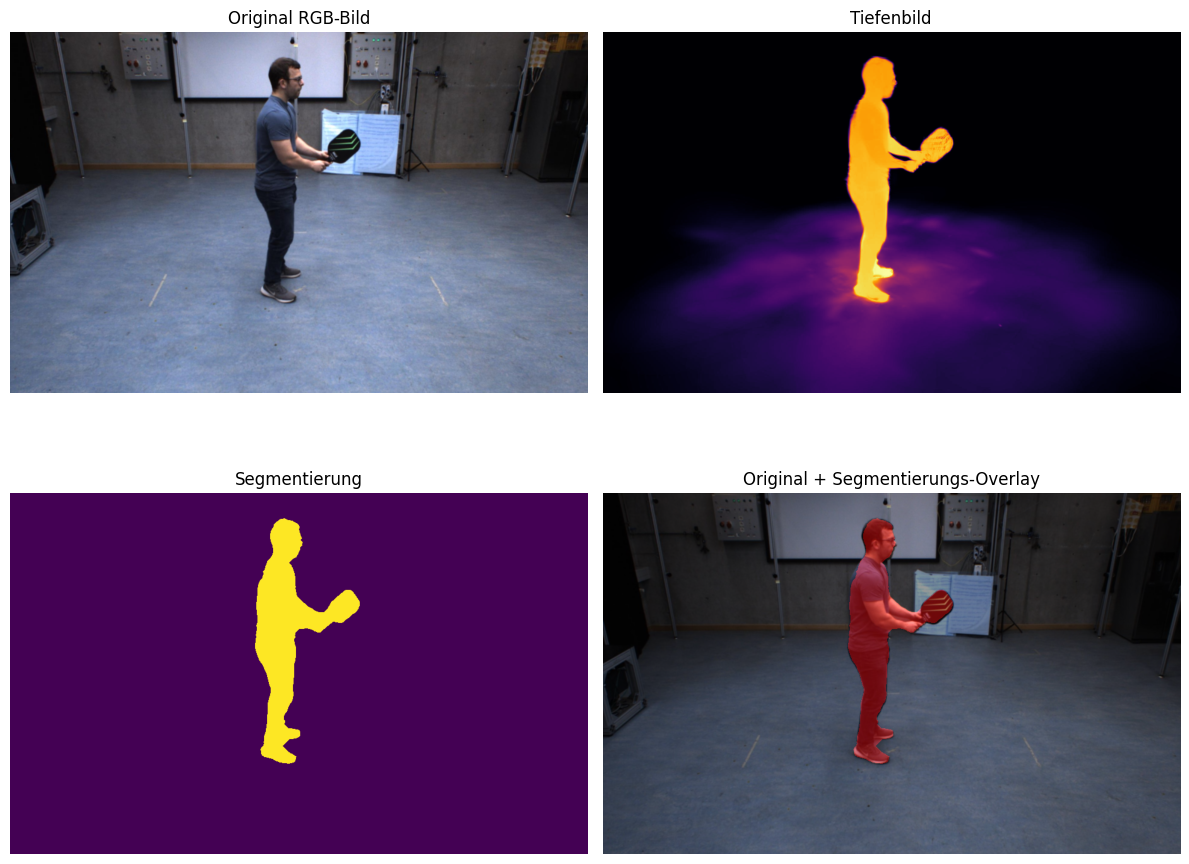
\includegraphics[width=1\linewidth]{bilder/Results/D3DGS/visualization_8.png}
%     \caption{Beispiel für die Maskenerzeugung: oben links Ground-Truth RGB, oben rechts gerenderte Tiefenkarte; unten die aus der Tiefenkarte abgeleitete Binärmaske nach Schwellenwertbildung und morphologischem Closing.}
%     \label{fig:Segmentation_D3DGS}
% \end{figure}


\subsection{Trainingsansätze}

Zunächst wurde das Modell mit dem im vorherigen Abschnitt beschriebenen, vorbereiteten Datensatz trainiert. 
In einem ersten Schritt kamen alle in der Originalimplementierung vorgesehenen Parameter und Verlustterme unverändert zum Einsatz. 
Dabei zeigte sich jedoch, dass insbesondere die zusätzlichen Kamera-Parameter \texttt{cam\_c} und \texttt{cam\_m}, welche Helligkeit und Kontrast der gerenderten Bilder steuern, die Farbdarstellung im NSTL stark verfälschten. 
Um eine stabilere Trainingsdynamik und konsistentere Farbtreue zu gewährleisten, wurden diese Parameter aus der Optimierung entfernt und stattdessen fixiert.  

Ein weiterer Anpassungsschritt betrifft den in der Originalarbeit enthaltenen sogenannten \emph{Floor-Loss}. 
Dieser bestraft Punkte, die unterhalb der Ebene $y=0$ liegen, und dient damit der Stabilisierung in Szenen mit bekanntem Bodenverlauf. 
Im NSTL verläuft die $y=0$-Ebene jedoch schräg durch den Raum, sodass der Verlust hier ungewollt auch relevante Vordergrundstrukturen bestraft hätte. 
Der Floor-Loss wurde daher vollständig deaktiviert. 
% Ein Plot zur Visualisierung dieses Problems befindet sich in Anhang~\ref{sec:appendix_floorloss}.  

% Die beschriebenen Anpassungen führten zu den bislang stabilsten Trainingsläufen. 
% Weitere Varianten – etwa eine Einschränkung des L1-Anteils im Bildverlust auf relevante Regionen – wurden konzeptionell vorbereitet, konnten im Rahmen dieser Arbeit jedoch nicht mehr umfassend untersucht werden.



% \subsection{Implementationsdetails}

% Welche Basis du übernommen hast (z. B. offizielle Implementierung von Luiten).

% Welche Parameter im Training angepasst wurden (Batchgrößen, Speichergrenzen, VRAM-Limit bei 50 Frames).

% Nutzung des festen Hintergrunds in Kombination mit Dynamic 3DGS.

% \subsection{Trainingsvarianten}

% Hier listest du nur deine Iterationen und Modifikationen, ohne das ganze Grundprinzip zu wiederholen:

% Entfernen von \texttt{cam_c} und \texttt{cam_m}.

% Entfernen des Floor Loss aufgrund schiefem Koordinatensystem.

% Unterschiedliche Initialisierungen: zufällige Punktewolke vs. PLY-Loader vs. mittlere Gaussians.

% Varianten mit/ohne Segmentierung.

% Nur mittlere Gaussians dynamisch, andere statisch.

% Daraus kannst du zwei Unterkapitel machen:

% Ablationsstudien (kurze Darstellung aller Varianten, ggf. Abbildung oder Tabelle mit qualitativen Beispielen, Hauptteil + Rest in Anhang).

% Optimale Konfiguration (die Variante, die im Rest der Arbeit verwendet wird).

% \subsection{Diskussion der Limitationen}

% Speichergrenze bei 50 Frames.

% Qualitäts-Tradeoff bei schnellen Bewegungen.

% Probleme mit Metriken, da Hintergrund nicht mitgerendert wird.




 % Externe Datei einbinden
\chapter{Methodology}

This chapter presents the complete methodology developed for constructing, combining, and rendering Gaussian Splatting models for both static and dynamic 3D scenes. 
The proposed system is designed to transform synchronized multi-view recordings into modular Gaussian representations and to recompose them into complex, synthetic environments. 
It consists of two main processing stages: \textbf{Pipeline A}, which reconstructs 3D and 4D Gaussian models from calibrated camera data, and \textbf{Pipeline B}, which composes these models into structured multi-object scenes for dataset generation. 
Together, these stages establish a unified framework that bridges real-world capture and synthetic data creation through differentiable Gaussian rendering. 
An overview of the entire process, including both reconstruction and composition stages, is illustrated in Figure~\ref{fig:Ablauf}.

\begin{figure*}[!t]
    \centering
    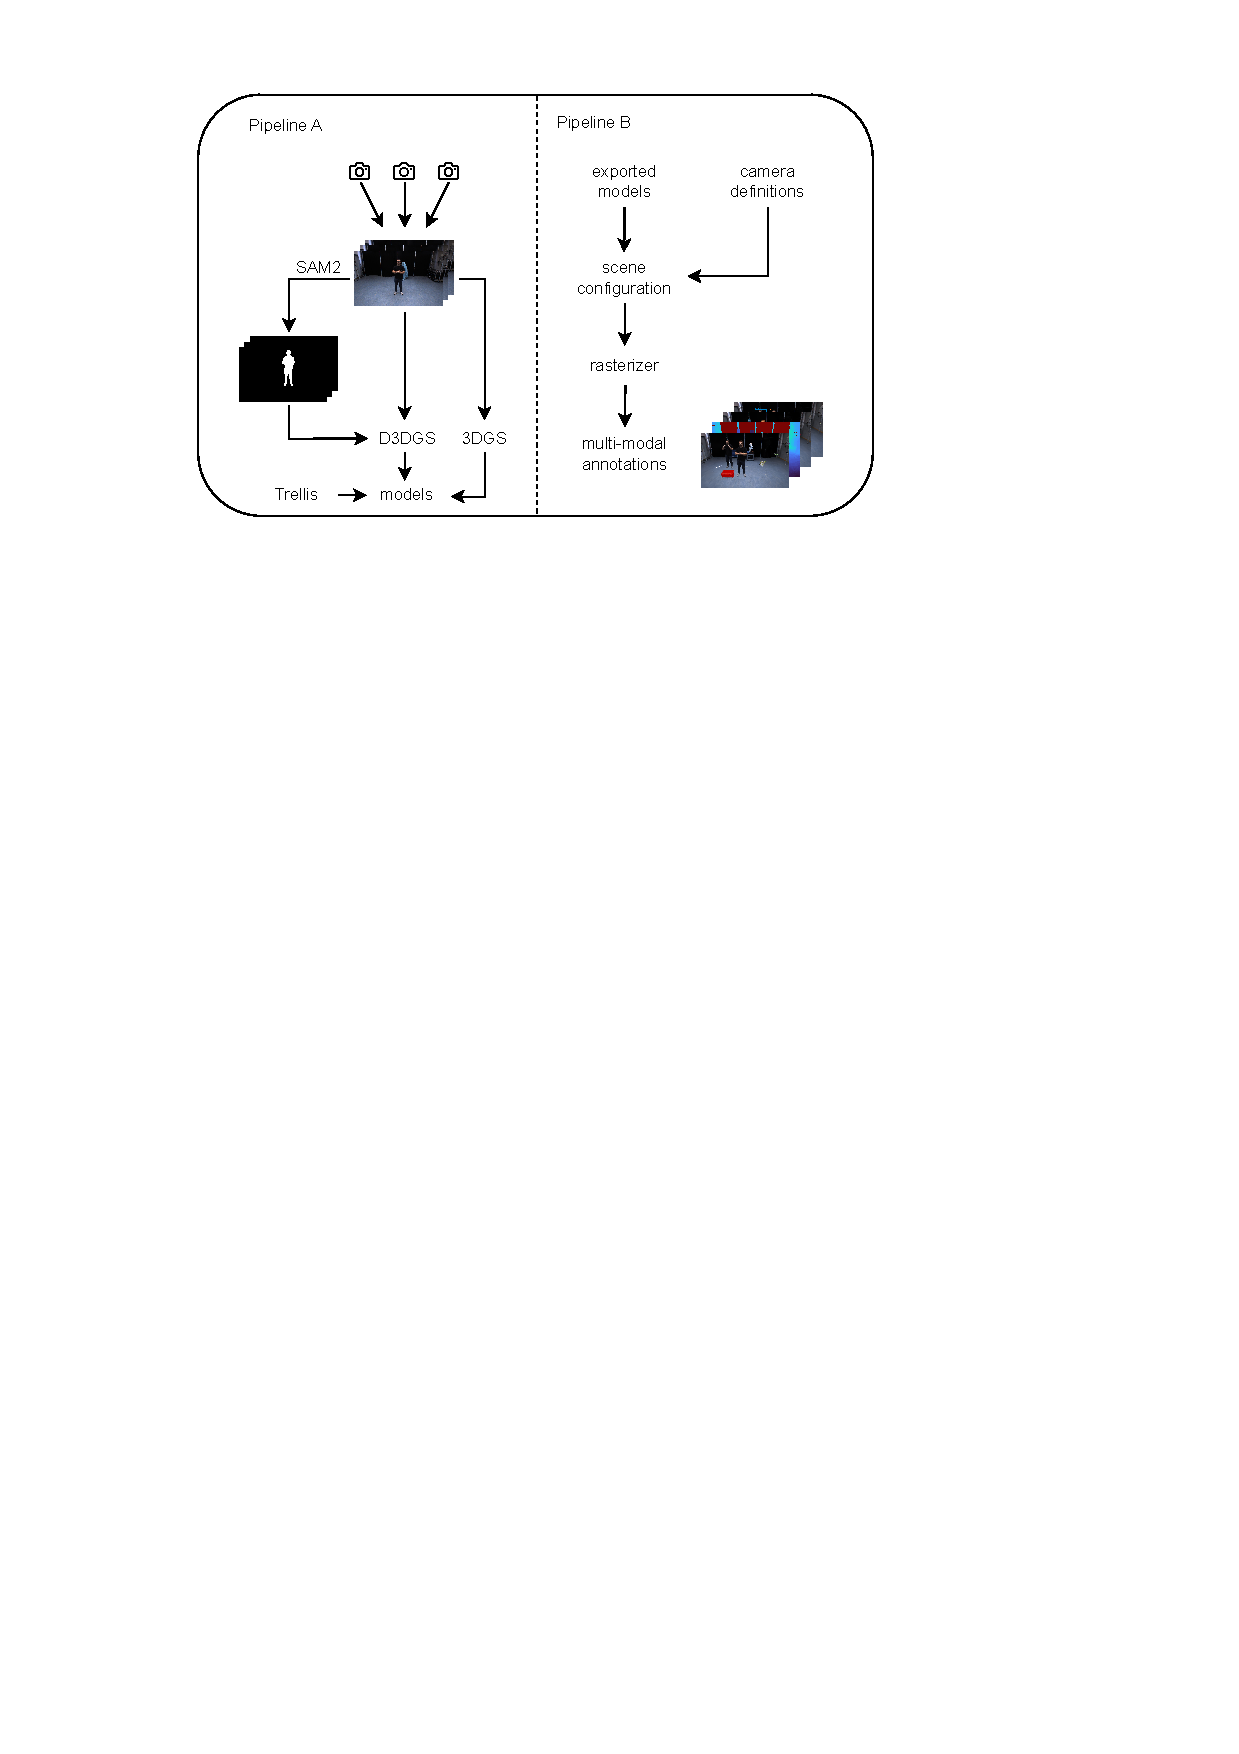
\includegraphics[width=0.9\textwidth]{Grafiken/Ablauf.pdf}
    \caption{
       \textbf{Overview of the proposed composition pipeline.}
        \textbf{Pipeline A} converts multi-view captures into per-object 3DGS and D3DGS models via calibration, mask generation, and model training.
        \textbf{Pipeline B} composes exported models into multi-object scenes, producing synchronized RGB, depth, segmentation, and occlusion annotations.
    }
    \label{fig:Ablauf}
\end{figure*}


\section{Pipeline A: Reconstruction of 3D and Dynamic 3D Models}

The first stage of the system, referred to as \emph{Pipeline A}, transforms synchronized multi-view image sequences into individual Gaussian Splatting models. It uses a high-density capture rig and follows four main stages: capture and calibration, preprocessing, mask generation, and model training.

\subsection{Capture setup and calibration}
The acquisition takes place in a custom-built multi-camera rig equipped with 56 globally synchronized cameras operating at a resolution of \(1920 \times 1200\) pixels and a frame rate of 30 frames per second. 
All cameras are connected to a shared hardware trigger that provides a global clock signal, guaranteeing microsecond-level temporal synchronization across all views.
The cameras are arranged in a hemispherical configuration around a capture volume of approximately \(1.5 \times 1.5 \times 2.5\) meters.
The geometric center of this volume serves as the global origin for all reconstructions.
This setup ensures dense overlapping views and uniform angular coverage, which are essential for complete and consistent 3D and 4D reconstructions.

Calibration is performed in two stages. Intrinsic parameters are estimated for each camera individually following the standard OpenCV pinhole model with five distortion coefficients \((k_1, k_2, p_1, p_2, k_3)\). The intrinsic model comprises focal length, principal point, and both radial and tangential distortion terms.
Because the optical center \((c_x, c_y)\) of each lens is not necessarily aligned with the image center, an \emph{optimal new camera matrix} is computed using OpenCV’s rectification routines to balance field of view and minimal distortion. This step yields undistorted, rectified images that serve as input for all subsequent stages.
Extrinsic calibration is performed once for the entire rig via a global optimization of inter-camera correspondences obtained from a moving checkerboard sequence. 
The resulting extrinsic parameters define all cameras within a unified world coordinate frame.  

\subsection{Data Preparation: Mask Generation and Prompt Propagation}
\label{sec:maskgen}

Dynamic 3D Gaussian Splatting requires per-frame object masks to disentangle dynamic objects from the static background and to maintain temporal consistency during training \cite{luiten2024dynamic}. While the reference implementation primarily relies on binary foreground/background masks, this pipeline extends that step by integrating \textbf{SAM2} \cite{ravi2024sam2}, enabling interactive prompting and high-quality instance segmentation across frames.

Segmentation is initialized by selecting a seed frame and providing manual point or box prompts for the objects of interest. These seed prompts are propagated across all cameras in the calibrated multi-view setup. Concretely, for each camera in the sequence the corresponding seed image is used to generate an initial segmentation prompt that is added to the predictor state, ensuring consistent initial object masks across views. Subsequently, masks are propagated temporally across the sequence using the SAM2 video predictor. This procedure yields temporally consistent, per-camera instance masks for all frames of the dataset. Compared to classical foreground/background segmentation, this approach permits fine-grained object delineation and is more resilient to occlusions and appearance changes across time and viewpoints. The resulting masks are fed directly into the D3DGS training pipeline to supervise dynamic object reconstruction.

\subsection{3D / Dynamic-3D Gaussian Model Training}
\label{sec:modeltraining}

Per-object Gaussian Splatting models are trained using the rectified images, calibrated poses, and instance masks. Static instances are reconstructed with 3DGS~\cite{kerbl3Dgaussians}; dynamic instances use persistent D3DGS~\cite{luiten2024dynamic}. 

The training procedure follows the original methods with two notable deviations. First, Gaussian positions are not initialized from sparse COLMAP point clouds. Because the multi-camera rig is pre-calibrated with known intrinsics and extrinsics, no additional SfM reconstruction is required for each scene. Instead, random point clouds are used to initialize each scene, significantly reducing overhead when training new sequences. Second, all reconstructions share a common global coordinate system, guaranteeing consistent alignment across different captures. Consequently, models trained in separate sequences can be merged directly without additional markers, manual registration, or extra calibration steps.

\paragraph{External 3D assets.}
In addition to models reconstructed with 3DGS and D3DGS, Pipeline A can incorporate externally generated 3D assets. To demonstrate this, small object models produced with \textbf{Trellis}~\cite{xiang2024structured} are used; Trellis reconstructs compact GLB meshes from a few input images and can export models as Gaussian representations. Exported Gaussian assets are imported without modification into the composition framework, demonstrating compatibility with heterogeneous 3D sources such as small household objects (e.g., boxes, plants, or tools).

\section{Pipeline B: Composition and Synthetic Dataset Generation}

While Pipeline A focuses on reconstructing individual static and dynamic Gaussian models, Pipeline B composes these models into coherent multi-object scenes. Pipeline B combines exported models, places them in calibrated virtual environments, and produces synchronized outputs such as RGB images, depth maps, and segmentation masks. The pipeline thus connects reconstruction and dataset generation by providing all necessary modalities for synthetic training and evaluation.

\subsection{Scene configuration and class indexing}
A synthetic scene is defined by a structured list of object instances, each associated with placement parameters and camera trajectories used for rendering. Every object model is assigned a fixed class index that remains consistent throughout the dataset. These indices, together with the scene configuration, are recorded in a JSON manifest that serves as the central reference for all annotations. Each instance also receives a unique identifier and a stable display color from a predefined palette, ensuring consistent instance-level segmentation across frames and scenes. Once configuration is complete, the scene can be rendered either from the physical rig cameras or from virtual viewpoints.

\subsection{Camera definition and interpolation}
The pipeline supports both real and virtual camera configurations. Rendering may be performed using the original rig calibration or via interpolated viewpoints that generate smooth camera paths. Physical camera poses are interpolated while averaging intrinsic parameters to obtain continuous motion through the virtual environment. Temporal supersampling can optionally create intermediate frames through sub-frame interpolation of the Gaussian parameters. This yields smoother apparent motion and higher effective frame rates, which are useful for generating realistic video sequences and temporally consistent annotations.

\subsection{Placement duplication and motion handling}
Objects are positioned in the global coordinate system using rigid transformations composed of translation, rotation, and uniform scaling. Dynamic models carry time-dependent Gaussian attributes and are rendered according to their internal trajectories. The system allows objects to be duplicated and repositioned while maintaining unique instance identifiers. This flexibility enables the creation of diverse scene configurations with varying spatial arrangements and interactions between static and dynamic elements. The same set of reconstructed assets can therefore be reused across many compositions without retraining or manual adjustment.

\subsection{Mask rendering and mask types}
During scene composition, each object is rasterized independently into an object identifier buffer while performing depth testing to ensure correct occlusion ordering. The system exports two complementary mask variants that support different training scenarios. The \emph{visible mask} contains only pixels that remain visible after depth compositing, while the \emph{complete mask} is obtained by rendering the object in isolation and thresholding its depth and alpha values. The complete mask therefore contains the full object silhouette, including regions that may be occluded in the final composition. Providing both mask types ensures compatibility with various downstream pipelines: some models require visible masks for instance segmentation, while others benefit from complete masks for occlusion-aware augmentation.

\paragraph{Occlusion scoring}
For each frame \(t\) and instance \(i\), an occlusion score is computed as
\[
s_{\mathrm{occ}}(t,i) = 1 - \frac{|V_{t,i}|}{|C_{t,i}|},
\]
where \(V_{t,i}\) and \(C_{t,i}\) denote the pixel counts of the visible and complete masks, respectively. The score ranges from 0 (fully visible) to 1 (completely occluded). Occlusion scores are stored in the JSON manifest and can be used for filtering, sampling, or weighting during downstream training.

\subsection{6D pose estimation}
For each object instance, a rigid transformation 
$T_{\mathrm{obj}\rightarrow\mathrm{cam}} \in \mathbb{R}^{4\times4}$ 
is estimated to map canonical object coordinates into the current camera frame. 
The translation component is derived from the displacement of the object centroid, 
computed either over all Gaussian means or a designated subset of anchor points:
\begin{align}
t &= \bar{x}_{t} - \bar{x}_{0}, \\
\bar{x}_{t} &= \frac{1}{|\mathcal{A}|} \sum_{i \in \mathcal{A}} x_i^{(t)}.
\end{align}

Rotational change is obtained from the per-anchor quaternions 
$q_i^{(t)} = (w,x,y,z)$ using Markley’s quaternion averaging method~\cite{markley2007averaging}. 
A mean quaternion is computed for both the reference and current frame:
\begin{align}
q^{(t)}_{\mathrm{mean}} &= 
\arg\max_{\|q\|=1} q^\top
\left(\sum_i q_i^{(t)} q_i^{(t)\top}\right) q,
\end{align}
and the relative rotation is given by
\begin{align}
q_{\Delta} &= q^{(t)}_{\mathrm{mean}} \otimes \overline{q^{(0)}_{\mathrm{mean}}}, \\
R_{\Delta} &= \mathrm{quat2mat}(q_{\Delta}).
\end{align}

The resulting rotation is combined with an optional initial alignment $R_0$, yielding
\begin{align}
R_{\mathrm{obj}} = R_{\Delta} R_0.
\end{align}

Finally, the object-to-camera transform is assembled as
\begin{align}
T_{\mathrm{obj}\rightarrow\mathrm{cam}} =
\left(T_{\mathrm{w}\rightarrow\mathrm{c}}^{-1}\right)
\begin{bmatrix}
R_{\mathrm{obj}} & \bar{x}_{t} \\
0 & 1
\end{bmatrix}.
\end{align}

This transformation represents a temporally consistent 6D pose estimate 
that captures the object’s centroid and orientation changes over time. 
Although these poses are not absolute ground truth, 
they provide reliable internal motion estimates that can be leveraged 
for downstream tasks such as motion tracking, pose refinement, or activity recognition.



\subsection{Keypoint detection and propagation}
The system generates 3D keypoints for each captured dynamic human model. Keypoints for each dynamic human model are initially detected in a reference frame using a Detectron2-based detector \cite{Detectron22020}. The rasterizer was extended to return per-pixel Gaussian indices, enabling tracking of keypoints over time by associating them with the Gaussians that influence the corresponding 2D pixel locations. To ensure temporal consistency across frames, 2D keypoints are reprojected into 3D using rendered depth maps together with camera intrinsics and extrinsics. These 3D points are subsequently updated in each frame according to the motion of the associated 3D Gaussians, ensuring that keypoints follow the dynamic objects throughout the sequence.

\subsection{Rendered outputs and metadata}
For each rendered frame and camera, the pipeline exports RGB images, depth maps, per-instance visible and complete masks, bounding boxes, and object metadata.
All outputs are indexed in a JSON manifest that stores camera parameters, object transformations, occlusion scores, and keypoints, ensuring consistent synchronization across modalities.
For validation and manual inspection the pipeline can additionally output diagnostic overlays such as mask overlays, rendered bounding boxes, and projected 6D poses and keypoints.

\smallskip
Together, these components form a unified, reproducible system for scene composition and dataset generation from modular Gaussian-based models.
 % Externe Datei einbinden
\chapter{Results}


\section{Model Evaluation}


\subsection{Comparison of Results in NSTL with COLMAP and OpenCV}

To validate the 3D Gaussian Splatting method in the Neural Space Time Lab (NSTL), a new dataset was captured and prepared using two different calibration approaches: COLMAP and OpenCV. 
The scene was trained, rendered, and evaluated using SSIM, PSNR, and LPIPS metrics to assess the impact of the calibration method on reconstruction quality, as described in the methodology section (Chapter~\ref{chap:Methodik}).

The results are summarized in Table~\ref{tab:3dgs_results_nstl}. 
Both calibration methods achieve high reconstruction quality, with COLMAP showing slightly better metric values. 
The differences can be attributed to the optimized estimation of camera poses through the structure-from-motion (SfM) procedure.

\begin{table}[h]
\centering
\caption{Comparison of metrics for the scene from the NSTL dataset.}
\label{tab:3dgs_results_nstl}
\begin{tabular}{lccc}
\toprule
& SSIM $\uparrow$ & PSNR (dB) $\uparrow$ & LPIPS $\downarrow$\\
\midrule
COLMAP & 0.931 & 35.58 & 0.18 \\
OpenCV & 0.927 & 34.56 & 0.252\\
\bottomrule
\end{tabular}
\end{table}

Figure~\ref{fig:3dgs_COLMAP} shows a visual comparison for the COLMAP-based reconstruction. 
The rendered image closely resembles the ground truth, with clear textures and edges in the central region, while slight blurring is visible near the floor and image borders.

Figure~\ref{fig:3dgs_opencv} presents the OpenCV-based reconstruction. 
Texture fidelity in the central region remains high, but quality decreases more noticeably toward the edges, particularly at the floor and in background elements such as a ladder.

\begin{figure}[h]
    \centering
    \subfloat[Ground Truth]{%
        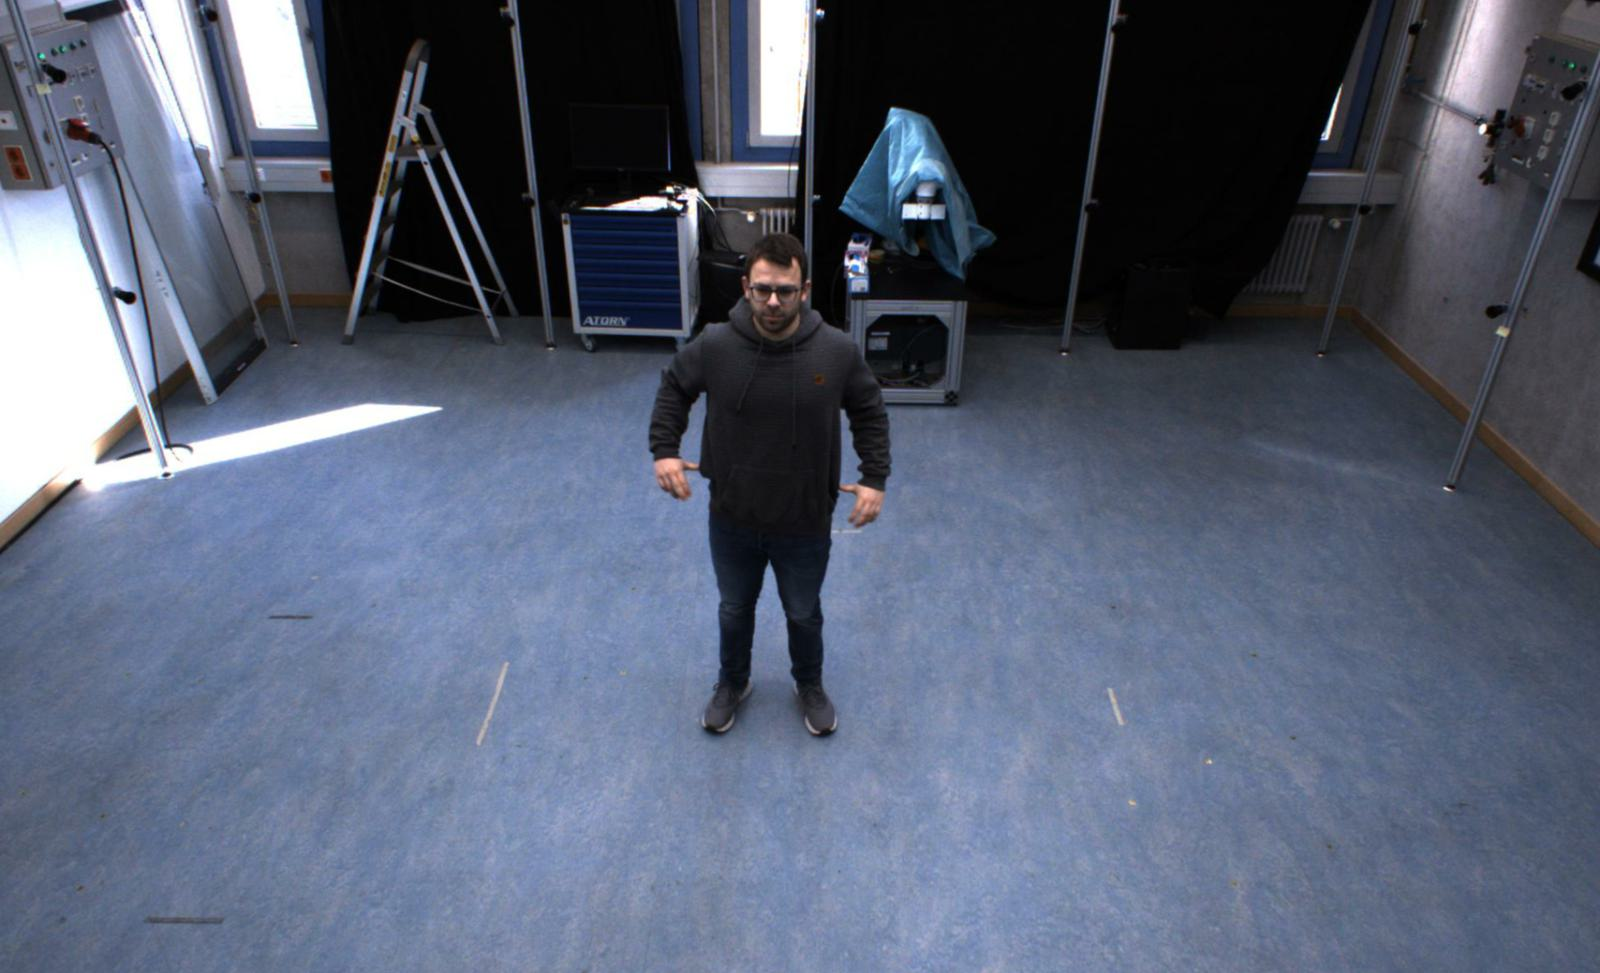
\includegraphics[width=0.48\linewidth]{bilder/Results/3dgs/3dgs_COLMAP_gt.jpg}%
    }
    \hfill
    \subfloat[Rendered Image]{%
        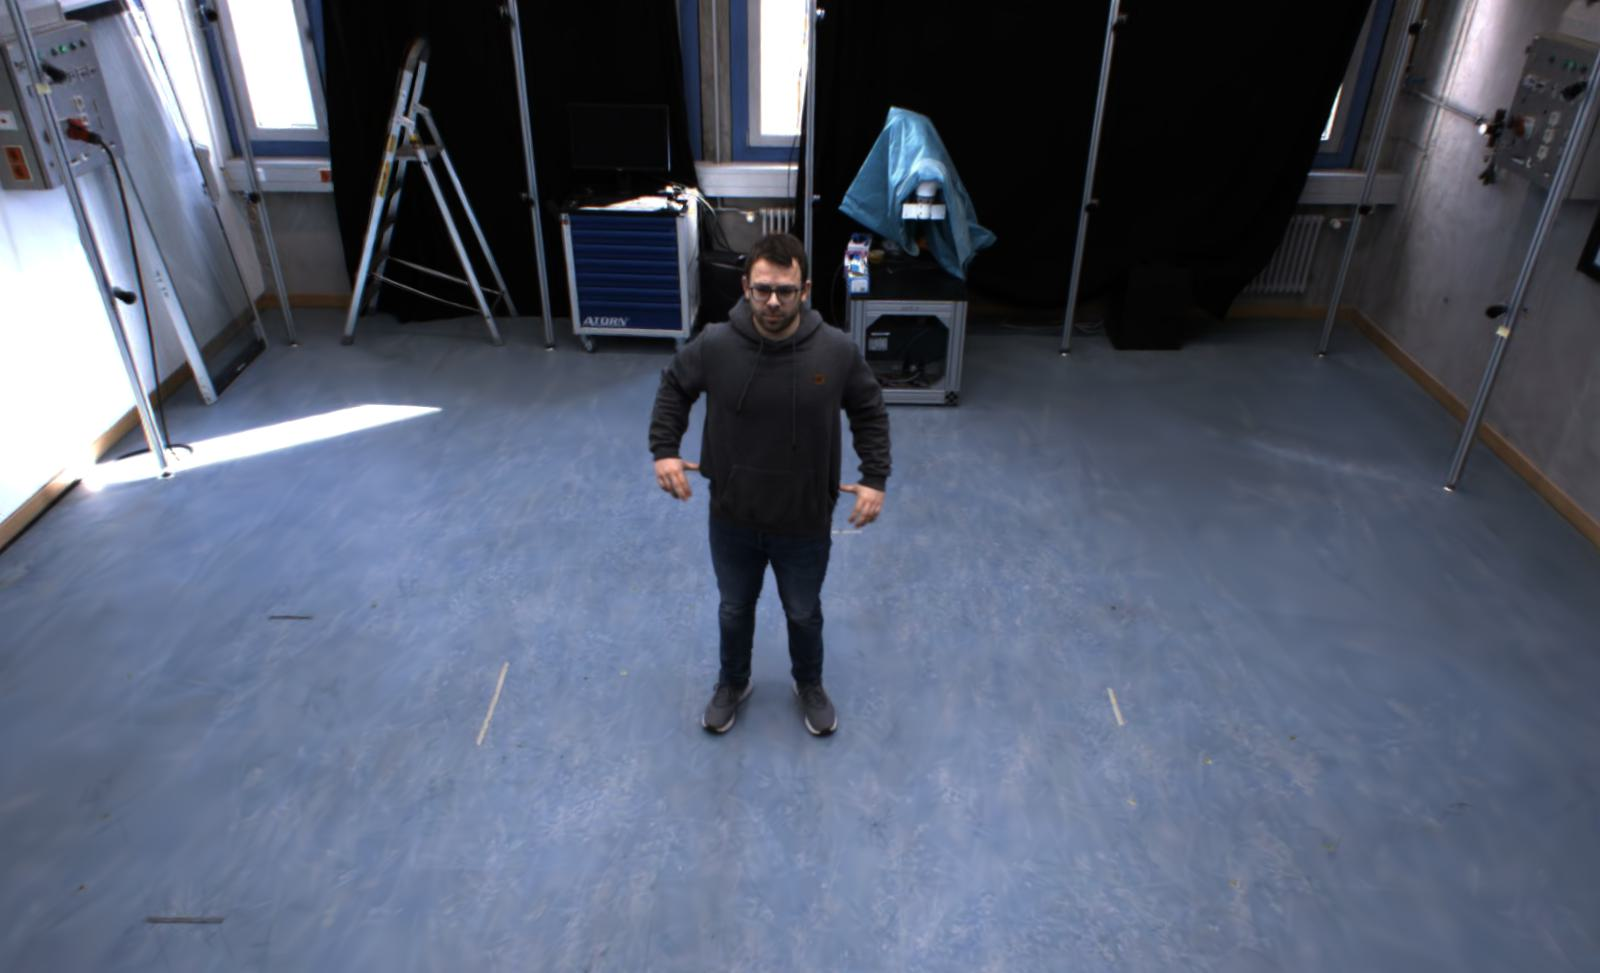
\includegraphics[width=0.48\linewidth]{bilder/Results/3dgs/3dgs_COLMAP_render.jpg}%
    }
    \caption{Comparison between ground truth and rendered image using COLMAP camera poses: The reconstruction shows clear textures in the central region, with minor blurring near the floor and image borders.}
    \label{fig:3dgs_COLMAP}
\end{figure}

\begin{figure}[h]
    \centering
    \subfloat[Ground Truth]{%
        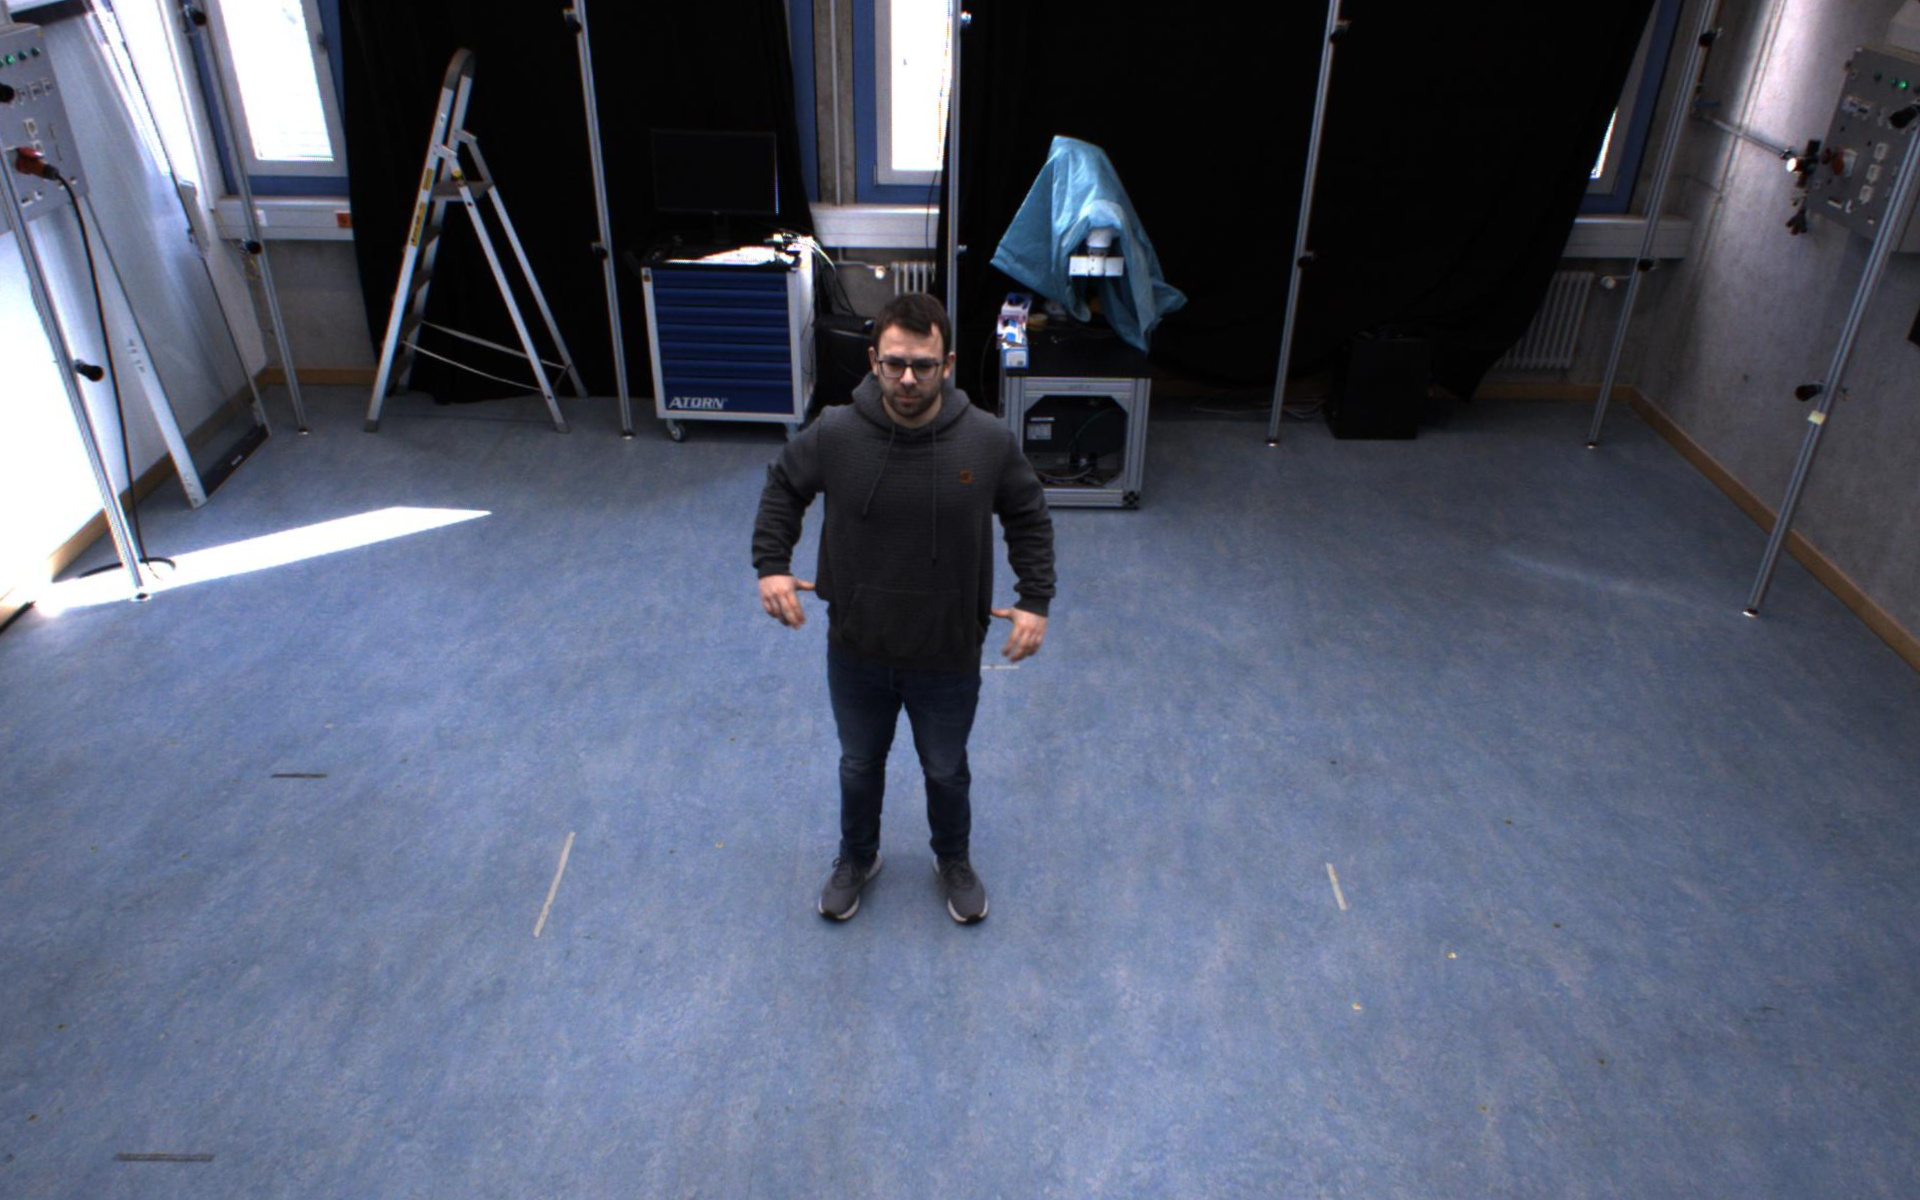
\includegraphics[width=0.48\linewidth]{bilder/Results/3dgs/3dgs_OpenCV_gt.png}%
    }
    \hfill
    \subfloat[Rendered Image]{%
        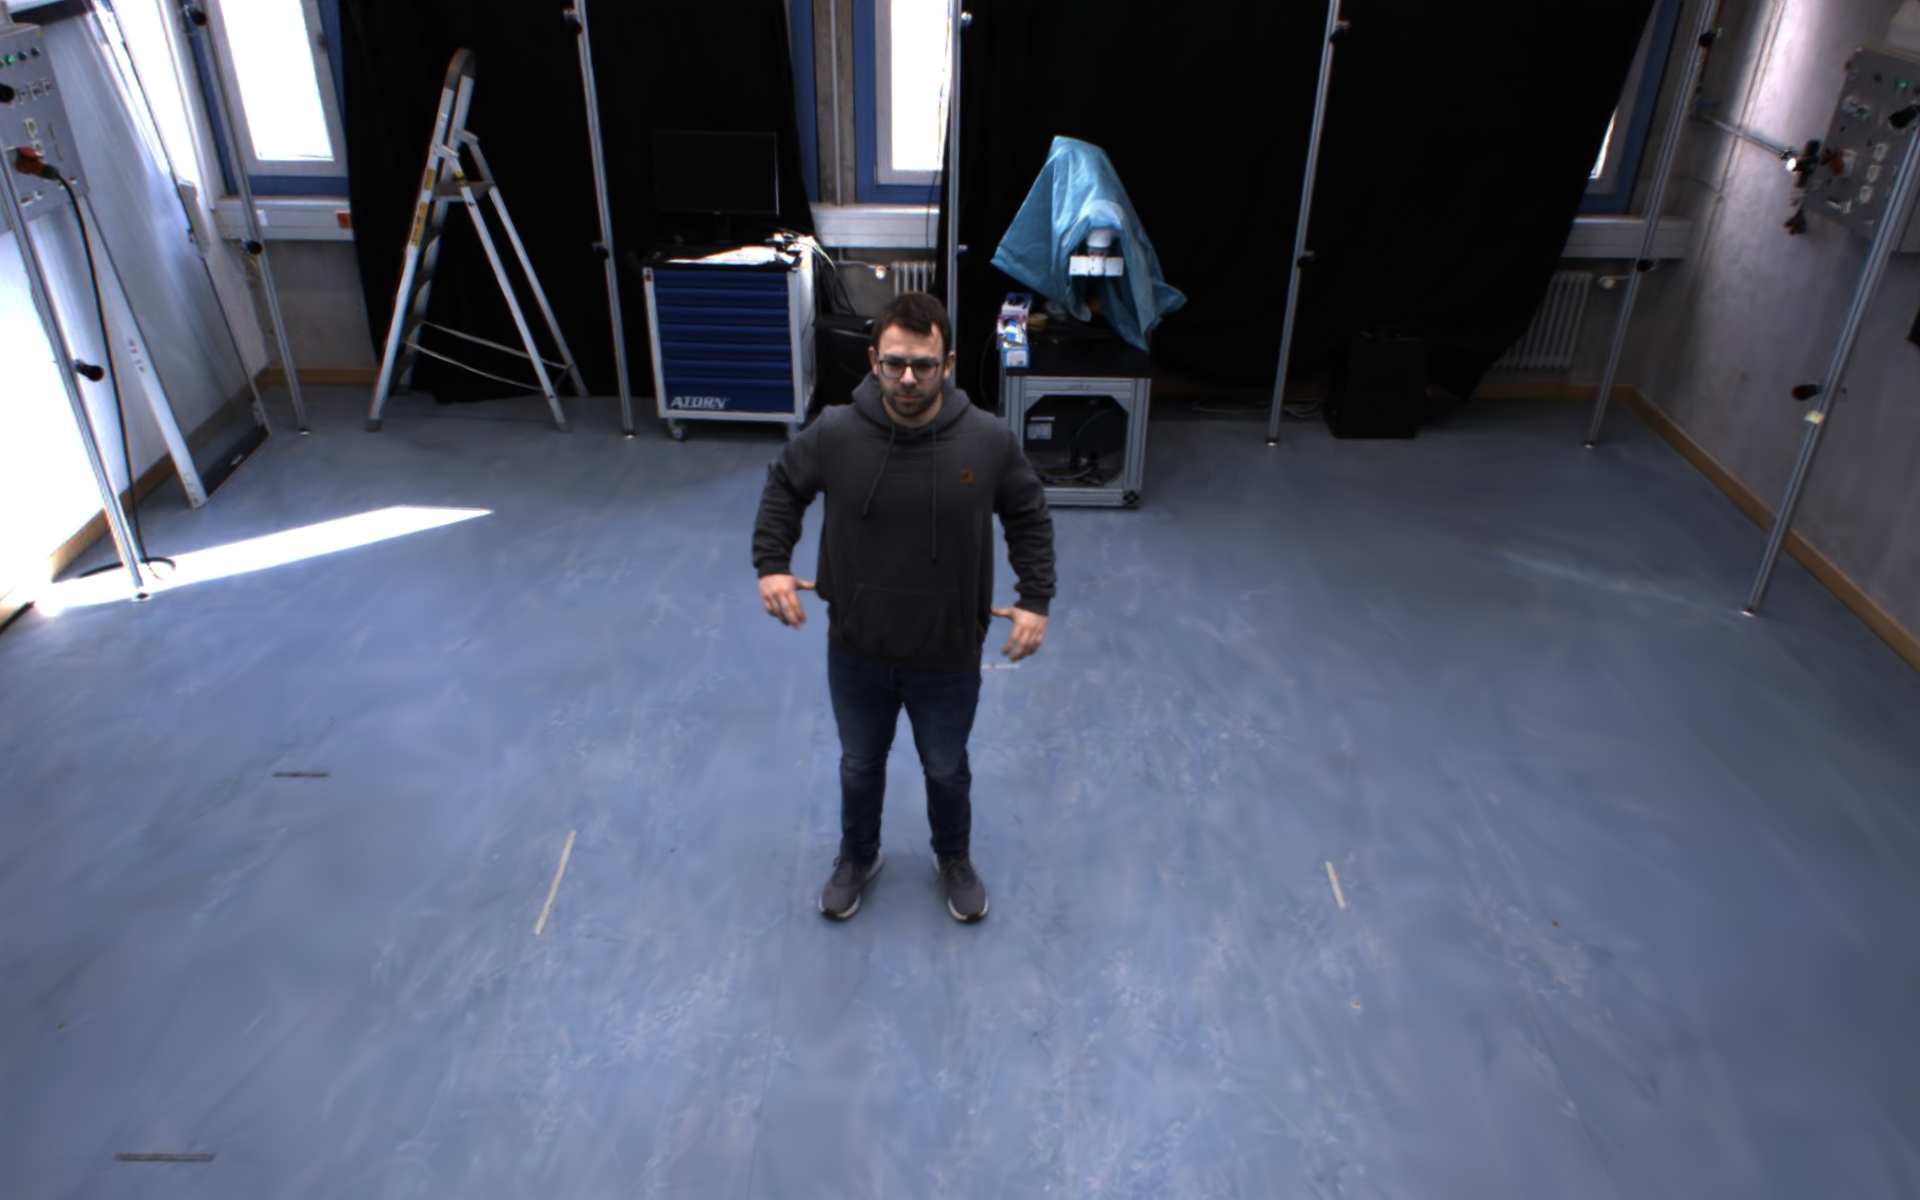
\includegraphics[width=0.48\linewidth]{bilder/Results/3dgs/3dgs_OpenCV_render.png}%
    }
    \caption{Comparison between ground truth and rendered image using OpenCV calibration: The reconstruction maintains good texture fidelity in the central region, with stronger blurring near the floor and background.}
    \label{fig:3dgs_opencv}
\end{figure}

Despite the slightly better metrics of COLMAP, OpenCV is preferred for NSTL applications, as explained in the methodology section (Chapter~\ref{chap:Methodik}). 
Deterministic calibration with OpenCV provides a coordinate system in real-world units, ensuring precise and reproducible spatial positioning. 
This is crucial for integration with other NSTL systems and for future extensions to dynamic scenes using 4D Gaussian Splatting. 
The similar reconstruction quality in the central region demonstrates that OpenCV, despite slightly lower metrics, is a robust alternative due to its consistency and lower dependence on scene-specific optimizations. 
These results provide a solid foundation for the investigation of dynamic scenes in the following sections.




\section{Composition Pipeline Evaluation}

This chapter presents a qualitative evaluation of the proposed multi-camera compositing and dynamic scene generation pipeline. 
In the absence of complete ground-truth annotations, the analysis focuses on visual consistency, temporal coherence, and scene-level generalization across multiple reconstruction and rendering configurations. 
All results were produced using the same calibrated multi-camera rig under identical rendering parameters, without manual post-processing unless explicitly stated.

\section{Compositional Scene Generation}
Figure~\ref{fig:composition} illustrates how the proposed compositing pipeline integrates multiple independently reconstructed Gaussian Splatting models into a single, globally aligned scene. 
Each row in the figure shows one configuration step, starting from a single-object placement and progressing toward increasingly populated scenes that combine both static and dynamic objects.
For each configuration, the corresponding RGB renderings, depth maps, bounding boxes, and segmentation overlays are presented to demonstrate multi-modal coherence.

A central advantage of the system is that all semantic annotations, including instance masks, class indices, and bounding boxes, are generated automatically and remain geometrically consistent across all rendered views. 
Since every 3D model is represented as Gaussian primitives within a shared coordinate system, mask generation requires no additional training or inference using segmentation networks. 
All semantic labels are deterministically derived from the compositing process itself, ensuring reproducible and noise-free annotations.

The modular design of the pipeline further enables high scene variability. 
Objects can be translated, rotated, scaled, or duplicated directly in 3D space without retraining or manual re-annotation. 
This flexibility allows large-scale dataset creation with controlled variation in object arrangement and spatial relationships. 
In practice, the same set of Gaussian models can be reused across numerous novel compositions while preserving consistent geometry, color, and semantic labeling, making the approach well suited for scalable and reproducible synthetic dataset generation.

\begin{figure*}[t]
    \centering
    \includegraphics[width=\textwidth]{Grafiken/Composition.pdf}
    \caption{
        \textbf{Compositional scene generation.}
        Example of multi-object scenes composed from independently reconstructed Gaussian Splatting models. 
        Each row shows one scene configuration with RGB, depth, bounding boxes, and segmentation overlays.
        All semantic annotations are generated automatically and remain spatially consistent across views.
    }
    \label{fig:composition}
\end{figure*}

\section{Multi-view Occlusion Handling}
To assess the robustness of the compositing mechanism under occlusions, 
Figure~\ref{fig:occlusion} shows segmentation overlays from two viewpoints of a scene containing interacting dynamic subjects. 
Even when large parts of one subject are occluded, the instance masks remain spatially consistent and tightly aligned with visible contours. 
This demonstrates that the rendering process preserves correct inter-object depth ordering and instance integrity across multiple perspectives. 
Such behavior is crucial for generating reliable training data for tasks such as instance segmentation or 3D scene understanding, where stable occlusion boundaries are essential.

\begin{figure}[ht]
    \centering
    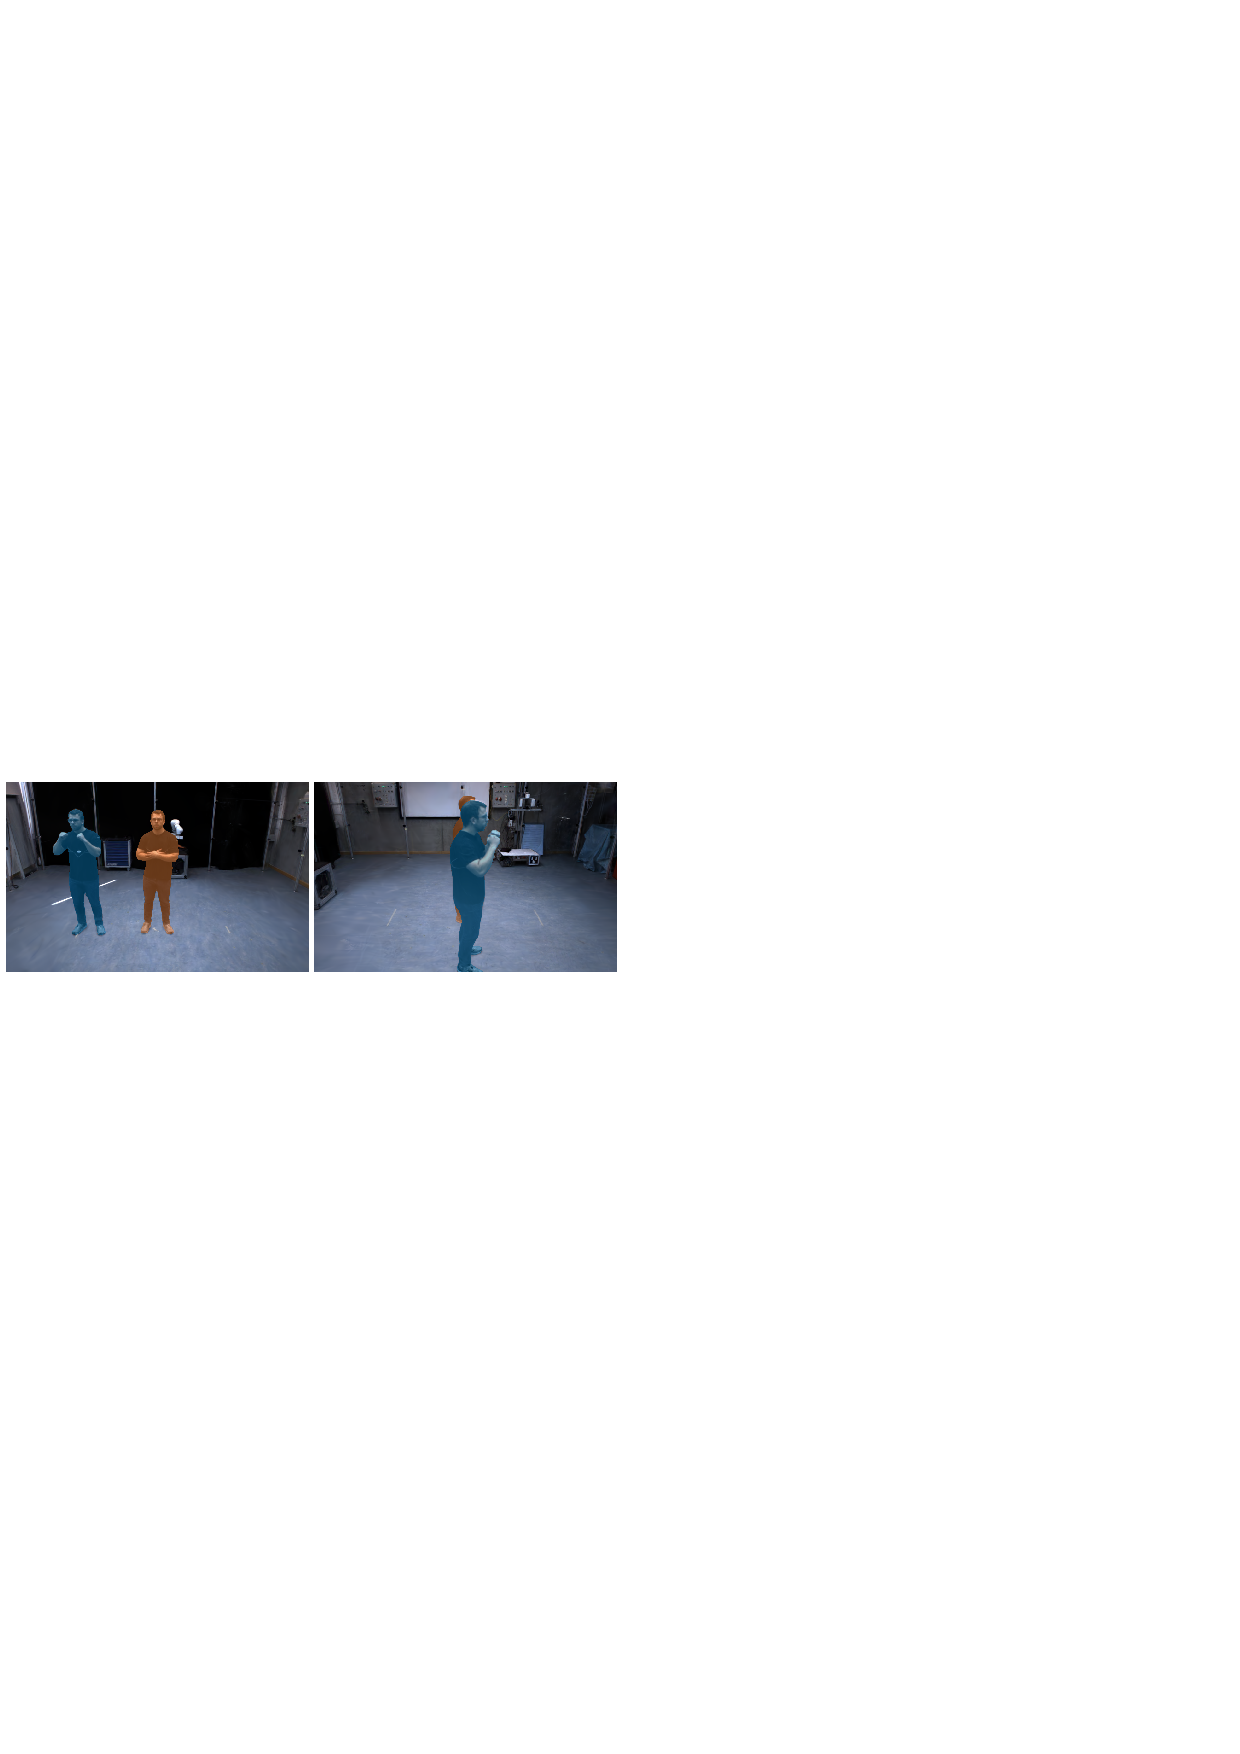
\includegraphics[width=\linewidth]{Grafiken/Oclusion.pdf}
    \caption{
        \textbf{Occlusion handling across views.}
        Segmentation overlays from front and side viewpoints of two interacting subjects.
        Even under strong mutual occlusion, instance masks remain consistent and well aligned with visible contours.
    }
    \label{fig:occlusion}
\end{figure}

\section{Scene Generalization}
Figure~\ref{fig:generalization} demonstrates the adaptability of the proposed system by recontextualizing dynamic subjects within a novel virtual environment reconstructed from real imagery using COLMAP \cite{schoenberger2016sfm}. 
The reconstructed environment provides realistic geometry and camera poses that serve as a spatial reference for compositing. 
Dynamic subjects are seamlessly integrated into the new setting, maintaining correct spatial alignment, depth consistency, and segmentation coherence. 
By decoupling object-level Gaussian models from a specific environment, the system enables arbitrary recombination of dynamic and static assets across scenes without retraining. 
This generalization capability supports large-scale variation in scene composition and facilitates applications such as domain adaptation, robustness evaluation, and synthetic-to-real transfer.

\begin{figure}[ht]
    \centering
    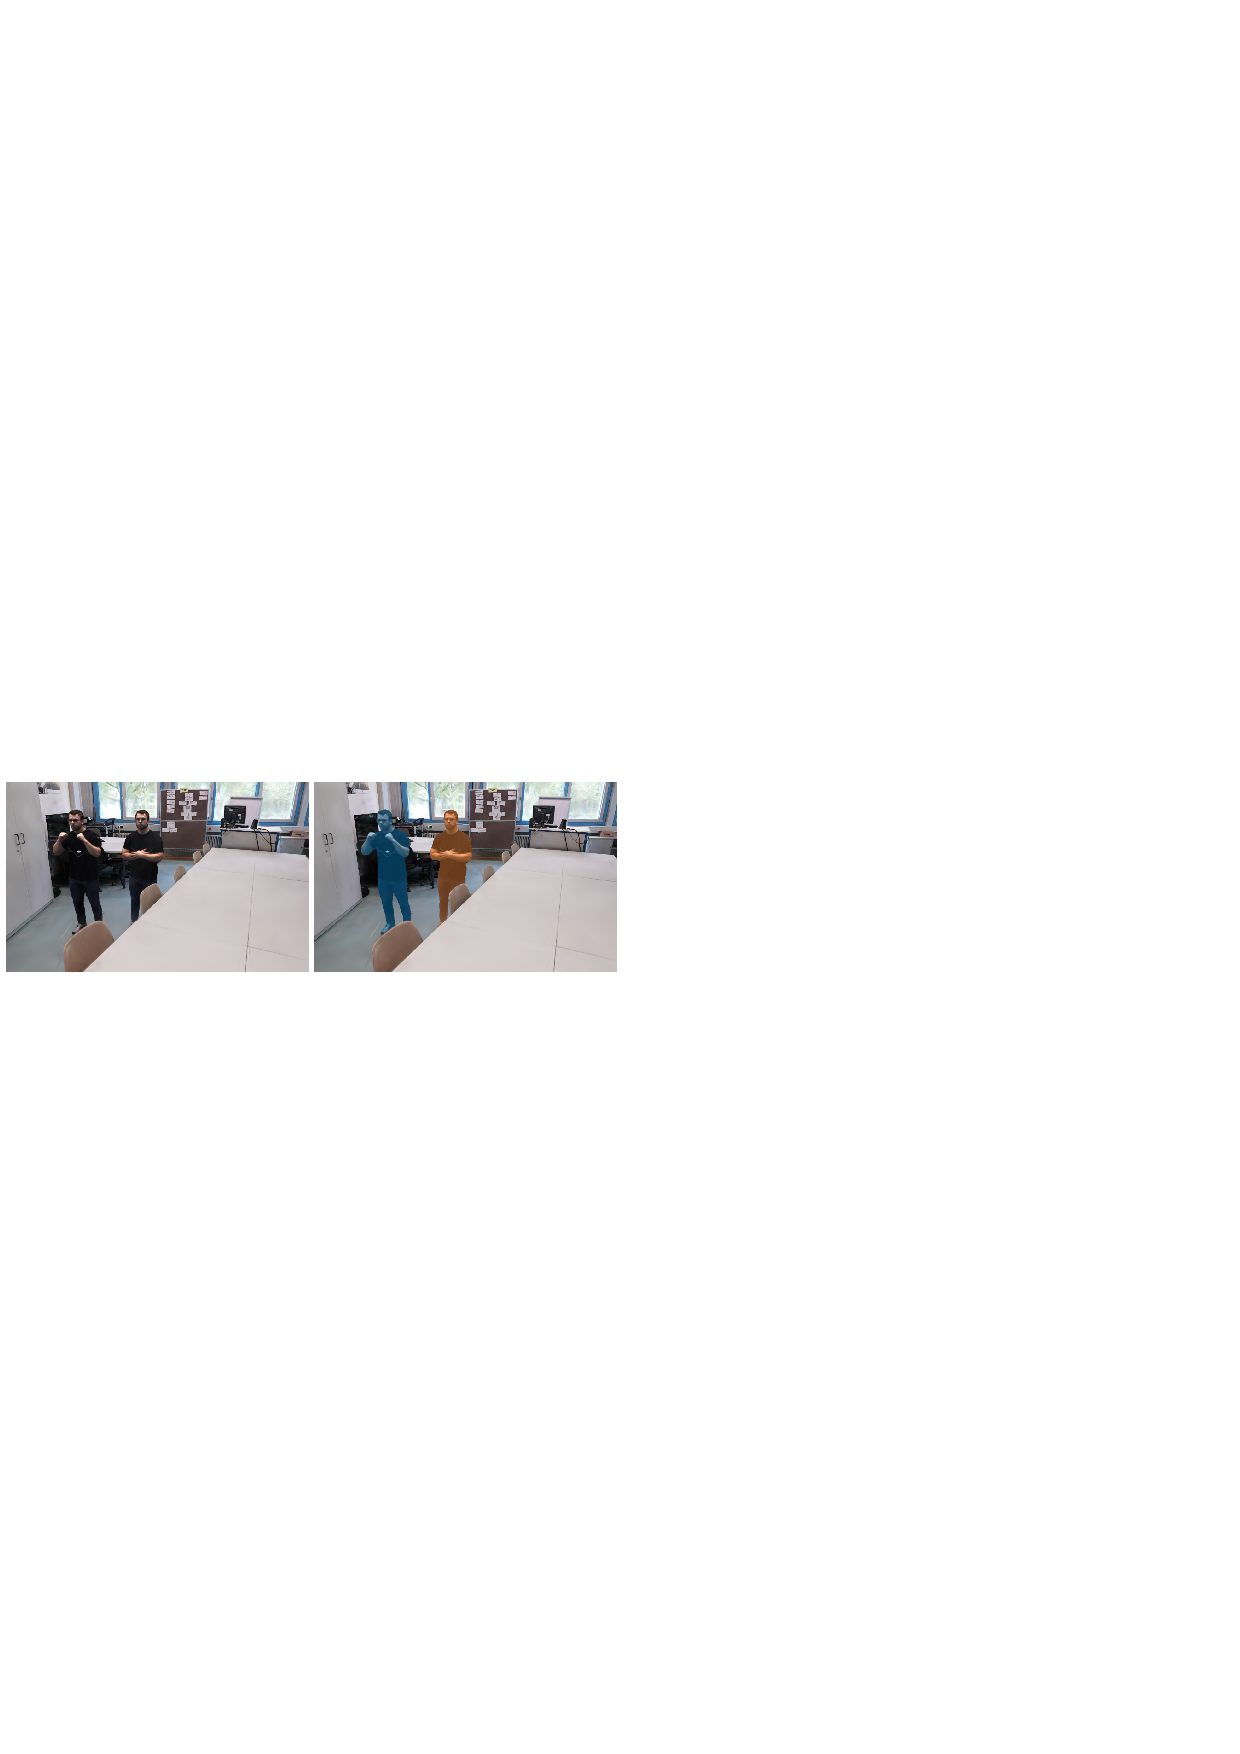
\includegraphics[width=\linewidth]{Grafiken/room_transfer.pdf}
    \caption{
        \textbf{Scene generalization and recontextualization.}
        Dynamic subjects composited into a novel virtual environment reconstructed with COLMAP.
        The system maintains consistent geometry and segmentation alignment across domains, 
        demonstrating flexible recontextualization of pre-trained Gaussian models.
    }
    \label{fig:generalization}
\end{figure}

\section{Temporal Consistency in Dynamic Scenes}
Dynamic scene rendering enables the generation of temporally coherent 4D datasets suitable for applications such as activity recognition, pose estimation, or motion segmentation. 
Figure~\ref{fig:temporal} shows representative frames from a dynamic sequence of a moving subject. 
The RGB and segmentation overlays reveal smooth and consistent motion over time, with stable geometry and accurate alignment across frames. 
Each time step preserves object structure and surface continuity, indicating that the Gaussian-based transformation updates produce interpretable and stable temporal behavior. 
This capability allows scalable synthesis of realistic dynamic sequences without requiring explicit motion capture or manual supervision.

\begin{figure*}[t]
    \centering
    \includegraphics[width=\textwidth]{Grafiken/time.pdf}
    \caption{
        \textbf{Dynamic scene generation.}
        Representative time steps of a moving subject with RGB and segmentation overlays.
        The consistent motion and geometry across frames demonstrate temporally stable 4D rendering.
    }
    \label{fig:temporal}
\end{figure*}

\section{Qualitative Pose Estimation}
Figure~\ref{fig:keypoints} (top row) shows qualitative 6D pose estimates for a dynamic human sequence across four time steps. 
Each frame visualizes the canonical object coordinate system derived from the aggregated Gaussian transformations. 
Although no ground-truth pose data are available, the estimated coordinate axes evolve consistently and reflect plausible orientation changes relative to the subject’s motion. 
This indicates that Gaussian-based transformation tracking provides a reliable approximation of object-level motion, suitable for downstream tasks such as pose refinement or motion analysis.

\section{Keypoint Propagation}
The lower row of Figure~\ref{fig:keypoints} visualizes the temporal keypoint propagation results obtained with a Detectron2-based detector \cite{Detectron22020}. 
Initial 2D keypoints are detected in a reference frame and projected into 3D by associating them with the nearest Gaussian centroids of the corresponding subject. 
As a result, keypoints are anchored on the object surface rather than the true anatomical joints, but they remain spatially coherent throughout the sequence. 
The keypoints are subsequently propagated in time according to the motion of the underlying Gaussians.

Temporal stability is observed across most body regions, particularly in the upper body where Gaussian density is high and motion is well captured. 
Minor deviations appear in areas with sparse or unstable Gaussian coverage, such as the knees or hips, leading to small temporal inconsistencies or spatial offsets. 
Despite these limitations, the propagation maintains overall semantic coherence and demonstrates that the Gaussian-based motion field can sustain meaningful correspondences over time. 
This behavior provides a promising foundation for future integration with articulated motion priors or learned joint-space constraints.

\begin{figure*}[t]
    \centering
    \includegraphics[width=\textwidth]{Grafiken/keypoints.pdf}
    \caption{
        \textbf{Qualitative analysis of pose and keypoint propagation.}
        Four frames of a dynamic subject showing estimated object poses (top) and propagated keypoints (bottom).
        The coordinate systems evolve consistently over time, while keypoint trajectories remain coherent despite local misalignments.
    }
    \label{fig:keypoints}
\end{figure*}

% \section{Summary}
% Overall, these qualitative results highlight that our framework can produce temporally stable geometric and semantic representations for dynamic scenes. 
% Although both pose and keypoint estimation currently rely on unsupervised tracking without ground-truth reference, the observed consistency across time demonstrates the potential of our 4D Gaussian representation as a foundation for future work in motion analysis, activity recognition, and articulated model learning.



 % Externe Datei einbinden
%\input{Kapitel/5_Comparison} % Externe Datei einbinden
\chapter{Summary and Outlook}

\section{Summary of Key Findings}

This work presented a modular and methodologically transparent pipeline for multi-view dataset generation based on static and dynamic 3D Gaussian Splatting representations.
Leveraging a purpose-built, hardware-synchronized multi-camera system, temporally aligned image sequences were captured from which both static (3DGS) and dynamic (D3DGS) models were reconstructed.
By integrating promptable segmentation (SAM2) and temporal mask propagation into the reconstruction workflow, all exported object models achieve geometric precision, temporal stability, and direct compatibility with downstream compositing.

A central contribution of the proposed system is the unified treatment of static and dynamic Gaussian models within a single compositional framework.
Pipeline~B enables deterministic scene assembly in calibrated camera rigs, producing spatially and temporally coherent outputs including RGB, depth, and instance-level masks.
By explicitly modeling occlusion, object placement, and temporal interpolation, the pipeline allows full control over rendered datasets while maintaining photometric and geometric realism.
This structure bridges the gap between reconstruction-focused Gaussian pipelines and practical dataset generation tools, supporting reproducible, multi-object scenes with synchronized multimodal annotations.

The framework further supports the seamless integration of externally generated 3D assets—such as those exported from \emph{Trellis}—demonstrating that pre-trained or lightweight 3D models can function as first-class entities within Gaussian-based rendering and composition.
As a result, the system generalizes across input modalities, accommodating both data-driven and generative 3D sources without modifications to the rendering logic.

\section{Limitations}

Despite its flexibility, several limitations should be acknowledged.
First, dynamic reconstructions rely on per-frame segmentation masks that, despite prompt propagation, may accumulate small temporal inconsistencies under strong occlusions or motion blur.
This can result in slight spatial drift of reconstructed Gaussians and propagated keypoints, particularly in regions with sparse Gaussian coverage such as knees or hips.

Second, although the compositional framework supports both static and dynamic elements, all rendered scenes currently assume rigid camera calibration and fixed illumination.
Consequently, phenomena such as global illumination, specular reflections, or cast shadows between independently rendered objects are not explicitly modeled, which can limit realism in certain composite configurations.

Third, pose estimation for dynamic objects is derived from Gaussian trajectories rather than explicit joint-based motion models.
While this approach ensures coherent motion propagation, it lacks semantic interpretability and may diverge from true skeletal motion.

Finally, the current implementation is optimized for controlled laboratory captures using pre-calibrated multi-camera rigs.
Generalizing to in-the-wild or handheld capture setups would require additional mechanisms to handle calibration drift, synchronization errors, and varying illumination conditions.

\section{Future Developments and Research Perspectives}

Several avenues remain open for further exploration.
A natural extension involves integrating articulated motion priors and skeleton-aware Gaussian tracking, which could improve alignment of dynamic keypoints and enable physically interpretable pose propagation.
Embedding such priors directly into the D3DGS training or composition stages may strengthen temporal coherence in regions with complex non-rigid motion, such as human limbs or deformable surfaces.

Another promising direction involves scaling the capture and synthesis process toward larger and more diverse datasets.
Automated scene composition, dynamic lighting control, and procedural environment synthesis could further enhance realism and diversity while maintaining annotation consistency.
In parallel, coupling Gaussian-based scene representations with diffusion-based appearance refinement or NeRF-style volumetric augmentation may bridge the remaining visual gap between synthetic and real-world imagery.

Finally, establishing standardized benchmarks for evaluating compositional and temporal consistency in Gaussian-rendered datasets would be highly beneficial.
Such benchmarks could promote reproducibility, enable quantitative analysis of temporal stability, and help define a common evaluation protocol for future research in Gaussian-based dataset generation.

Overall, this work demonstrates that temporally consistent Gaussian representations—when combined with geometry-aware compositing and transparent annotation pipelines—provide a practical and extensible foundation for the next generation of large-scale, multi-view training datasets. % Externe Datei einbinden
%\input{kapitel/kapitel5} % Externe Datei einbinden

\newpage

% Listen wenn überhaupt ans Ende und nicht an den Anfang.
% Meist ist das aber unnötig.
% \listoffigures % Liste der Abbildungen 
% \listoftables % Liste der Tabellen
% \newpage

% % List of Figures
% \addcontentsline{toc}{chapter}{List of Figures}
% \listoffigures

\cleardoublepage

\bibliographystyle{plain} % Literaturverzeichnis
% \bibliography{references}

\begin{btSect}{thesis} % mit bibtopic Quellen trennen
\addcontentsline{toc}{chapter}{References}
% \markboth{References}{References}
\section*{References}
\btPrintCited
\end{btSect}







% Listen wenn überhaupt ans Ende und nicht an den Anfang.
% Meist ist das aber unnötig.
% \listoffigures % Liste der Abbildungen 
% \listoftables % Liste der Tabellen
% \newpage

% \bibliographystyle{plain} % Literaturverzeichnis
% \bibliography{references}


% \cleardoublepage
% \phantomsection
% \addcontentsline{toc}{chapter}{List of Tables}
% \listoftables

% Abbildungsverzeichnis erzeugen
% \cleardoublepage
% \phantomsection
% \addcontentsline{toc}{chapter}{List of Figures}
% \listoffigures

% \cleardoublepage
% \begin{btSect}{thesis} % mit bibtopic Quellen trennen
% \addcontentsline{toc}{chapter}{References}
% \section*{References}
% \btPrintCited
% \end{btSect}

% \addchap{List of Abbreviations}
% \begin{acronym}[D3DGS] % Die längste Abkürzung hier einfügen, um den Platz für die Abkürzungen zu reservieren
\acro{NeRF}{Neural Radiance Fields}
\acro{iNGP}{instant Neural Graphics Primitives}
\acro{IPE}{Integrated Positional Encoding}
\acro{MSE}{Mean Squared Error}
\acro{MLP}{Multilayer Perceptron}
\acro{MVS}{Multi-View Stereo }
\acro{NSTL}{Neural Spacetime Lab }
\acro{PDF}{Wahrscheinlichkeitsdichtefunktion}
\acro{3DGS}{3D Gaussian Splatting}
\acro{4DGS}{4D Gaussian Splatting}
\acro{D3DGS}{Dynamic 3D Gaussian Splatting}
\acro{PSNR}{Peak Signal-to-Noise Ratio}
\acro{ReLU}{Rectified Linear Unit}
\acro{SfM}{Structure from Motion }
\acro{SSIM}{Structural Similarity Index Measure}


\end{acronym}


% Tabellenverzeichnis erzeugen


% dann mit "bibtex thesis1" und "bibtex thesis2" arbeiten

\end{document}

;;; Local Variables:
;;; ispell-local-dictionary: "de_DE-neu"
;;; End:
